\section{Background}
This section of the thesis introduces the key concepts related to the field of study. The section mainly discusses neural networks, object detection, transfer learning and domain adaptation. Additionally, the section will familiarize the reader with the relevant terminology and notations used. Furthermore, this section will briefly introduce the state-of-the-art industrial object detectors. The section will provide an extensive overview of the latest domain-adaptive object detection methods. Finally, the topic of  continual learning will be introduced. 
\subsection{Deep learning and neural networks}
Historically, machine learning(ML), a sub-field of Artificial Intelligence(AI), has been a highly computational task. The primary cause of it was linked to low hardware performance. According to Moore's law \cite{Etiemble2022}, the amount of transistors doubles in a circuit in a given number of months.  As the computational power of the computers grew proportionally to the number of transistors, the results have been steadily improving. The improvement was further facilitated with the discovery of the Graphical Processing Unit(GPU) applicability in ML tasks \cite{Hwang2018}. Additional critical bottlenecks in ML were caused by sub-optimal algorithms and data availability limitations. As the availability of data improved, new fields of applications arose. These and many other advancements made it possible to accelerate the training speed of deep neural networks(DNN).  

\begin{figure}[htb]
	\begin{center}
		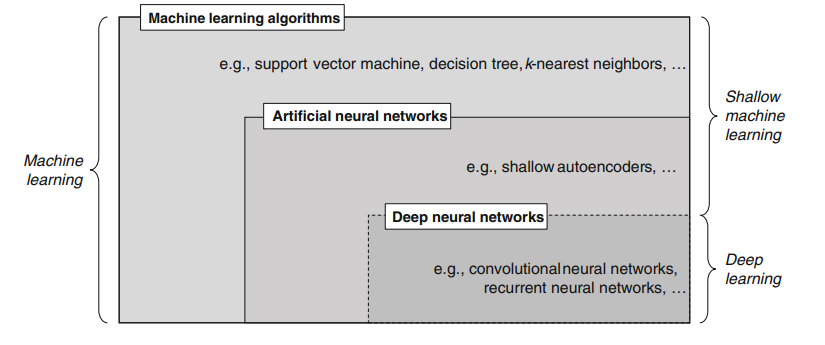
\includegraphics[width=0.8\textwidth,height=50mm]{./ml1.png}
	\end{center}
	\caption{Machine learning concepts \cite{Janiesch2021}.}
	\begin{center}
		\label{MLConcepts}
	\end{center}
\end{figure}
\FloatBarrier

The concept of deep neural networks originates from biology, where a network of neurons is fundamental to the functionality of a brain. In overly simplified terms, such network consists of interconnected neurons that capture an external signal and produce a certain reaction within the brain as a response. Figure \ref{NeuronSchem} (a) illustrates a typical neuron, where the signal flows from dendrites through the cell-body of the neuron. If the signal is strong enough, the neuron activated and passes the signal further to other neurons through the connections called "synapses", as shown in Figure \ref{NeuronSchem} (c). Identical process takes place in remaining neurons, which ultimately forms a neural network \cite{Mehlig_2021}.

\begin{figure}[htb]
	\begin{center}
		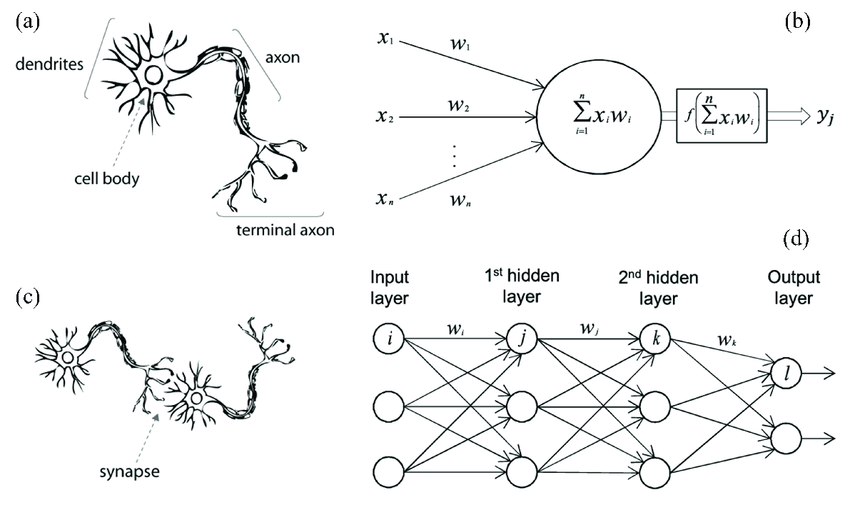
\includegraphics[height=8cm]{./BioNeuronVsArtificial.png}
	\end{center}
	\caption{A biological(a) neuron against artificial(b) and biological synapse(c) against artificial(d) \cite{article1}.}
	\begin{center}
		\label{NeuronSchem}
	\end{center}
\end{figure}
\FloatBarrier

In deep learning(DL), a sub-field of ML, this architecture has been borrowed to implement an artificial neural network(ANN), where a neuron is simply a unit that processes an input signal. Figure \ref{NeuronSchem} (b) demonstrates a simplified structure of an artificial neuron. Here, $x_1, x_2..x_n$ represent input signals, while $\mathcal{W} = w_1, w_2, ... w_n$ are the weights of the signal and $y_i$ is the output of the neuron. The higher the weights of the input are, the stronger the influence of the neuron on the output. The weighted sum of the inputs is then passed to the activation function, which essentially determines the output of the node and ultimately allows to learn complex patterns in data \cite{Mehlig_2021}. 

A few of the most popular non-linear activation functions include a logistic sigmoid, tanh function, softmax and a rectified linear unit(ReLU). Among the four, ReLU has been considered state-of-the-art in the field of deep learning due to the performance in convolutional neural networks(CNN) \cite{Dubey2021} and the simplicity. The logic of ReLU can be represented as follows: 
  
\begin{equation}
	\operatorname{ReLU}(x)=\max (0, x)= \begin{cases}x, & \text { if } x \geq 0 \\ 0, & \text { otherwise }\end{cases}
\end{equation}

Consequently, the output of the activation function is passed to a hidden layer of neurons, as illustrated in Figure \ref{NeuronSchem} (d). The layers in the middle are called "hidden" due to the fact that both outputs and inputs are masked by the activation function.  The hidden layers will calculate the weighted output of the previous layers until the signal eventually reaches the final output layer of the network. Hidden layers that stack up together to form a classical deep learning architecture \cite{OShea2015}. Such architecture allows to process data in a non-linear pattern. In the original ANN all the layers are fully-connected(FC), meaning that each node of the input vector affects each node of the output vector, as shown in Figure \ref{NeuronSchem} (d).


Due to the biological nature, neural networks adapt over time by creating new connections between neurons. The neurons in ANN adopted such behaviour by utilizing a backpropogation algorithm \cite{Rumelhart:1986we}. A naive backpropogation approach is illustrated in Figure \ref{fig:backprop}. The algorithm consists of two parts: feed-forward and backward loops. Generally, the main objective of an ANN is to choose such weights that the network produces desired target outputs. The forward pass propagates along the nodes in each layer of the neural network and returns a predicted output. In order to evaluate the quality of the predicted output, it is compared to the target output by using a cost(loss) function. The classic example of a cost function is a mean-squared error (MSE), which is commonly used in regression based problems. The equation to MSE is shown in Equation \ref{MSE_eq}.

\begin{equation}\label{MSE_eq} 
{\operatorname{argmin}} \frac{1}{n} \sum_{i=1}^{n}\left(f\left(x_{i}\right)-y_{i}\right)^{2}
\end{equation}

The MSE cost function attempts to minimize the distance between the predicted output and the target output, while giving more weight to larger distances due to the squared output \cite{Albarghouthi2021}.


\begin{figure}[htb]
    \centering
    \subfloat{{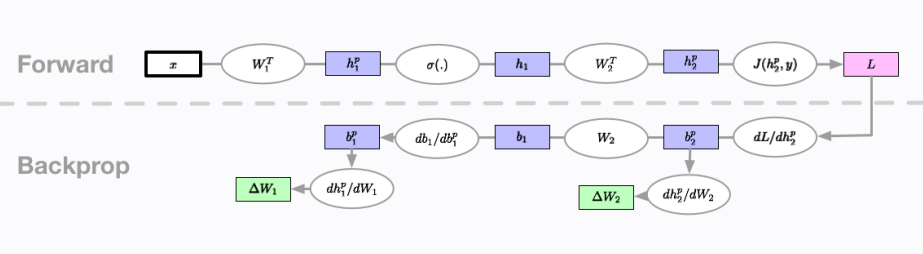
\includegraphics[width=10.5cm]{./Backprop1.png} }}%
    \qquad
    \subfloat{{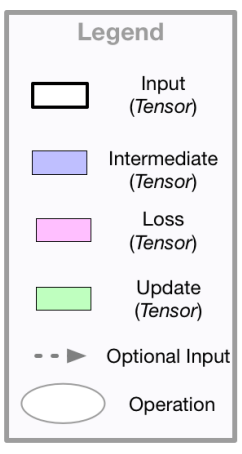
\includegraphics[width=1.5cm]{./Backprop2.png} }}%
    \caption{Backpropogation algorithm, adapted from \cite{Alber2018}.}\label{fig:backprop}%
\end{figure}
\FloatBarrier

In order to minimize the loss function, the algorithm calculates the partial derivative of the loss term $\mathcal{L}$ with respect to the weights: $\nabla g = \frac{\partial \mathcal{L}(f(x_i), y_i)}{\partial \mathcal{W}}$. The basic algorithm of the gradient descent is commonly used in optimizing such functions and its logic can be generalized as follows: 

\begin{enumerate}
  \item Initialize the algorithm with a random value of $\theta^{i}$, where starts with $i=0$.
  \item Define the next $\theta$ value as $\theta^{i+1} = \theta^{i}-\eta\left((\nabla g)\left(\theta^{i}\right)\right)$.
  \item Iterate over the values of $i$ and repeat until convergence \cite{Albarghouthi2021}.
\end{enumerate} 

Generally speaking, there are three gradient descent algorithms: batch gradient descent, stochastic gradient descent(SGD) and mini-batch gradient descent. While the batch gradient descent updates the model only after all the samples have been evaluated, the SGD calculates the error for one sample in the dataset and updates the parameters one by one. On the other hand, the mini-batch gradient descent algorithm splits the data into smaller batches and calculates updates on each of the data subsets. 

Finally, by applying the chain rule to the derivatives in a backwards-direction, the updates for the matrix $\mathcal{W}$ are calculated for the nodes in the neural network \cite{Alber2018}. The algorithm is then repeated until the global minimum is reached. The process of determining the weight values to utilize in each subsequent layer in the neural network by means of backpropogation algorithm is called "training the model". During training, the value that $\Delta W$ are updated is known as "learning rate" (LR). This hyperparameter of the network typically equals to a small value between 0 and 1. Picking too high LR value would result in overshooting e.g. never finding the global minimum, while too low value will lead to slow convergence and higher computational costs. 


\subsection{Neural networks in computer vision}
\label{neural_nets} 
With the discovery of DNN, many of the popular computer vision techniques became obsolete. Specifically, the introduction of CNNs was an important milestone in boosting machine perception performance \cite{Mahony2019}. Nowadays, CNNs are typically used to address various pattern recognition and computer vision tasks. Some of the tasks  include:

\begin{itemize}
	\item Image Classification
	\item Object Detection
	\item Segmentation
	\item Facial Recognition
	\item Domain Adaptation
	\item Image Reconstruction
	\item and many others \cite{paperswithcode:2022}
\end{itemize}

For addressing the key objectives of this work (Section \ref{objective}), the thesis will extensively cover image classification, object detection and domain adaptation tasks. Figure \ref{CNN} illustrates a simplistic CNN architecture approach to the MNIST  \cite{lecun-mnisthandwrittendigit-2010} classification problem. A CNN is essentially a neural network that leverages convolutional layers to produce predictions. Unlike the traditional computer vision methods, CNNs do not need to extract features of the image beforehand due to the logic behind convolution. In classical ML the features are extracted separately, followed by the appropriate algorithms for learning. On the contrary, DL algorithms, such as CNN, learn the features automatically \cite{alom01}.


\begin{figure}[htb]
	\begin{center}
		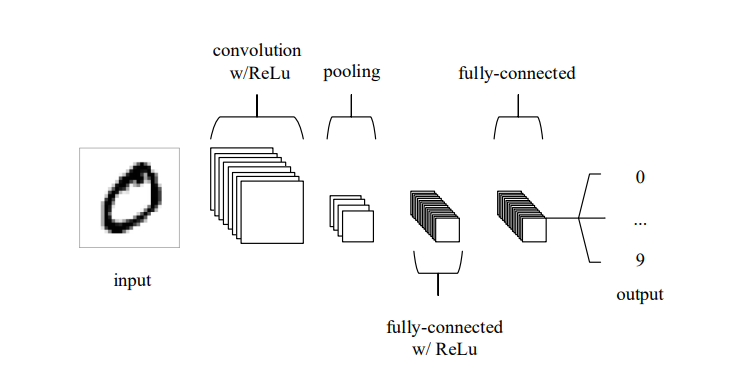
\includegraphics[height=5cm]{./CNN.png}
	\end{center}
	\caption{A simple CNN network with 5 layers for image classification task \cite{Mahony2019}.}
	\begin{center}
		\label{CNN}
	\end{center}
\end{figure}
\FloatBarrier

To understand the logic behind convolutional layers, it is important to discuss the operation of convolution. Convolution is a mathematical operation of two functions that indicates how the shape of one affected by another. In terms of image processing, convolution is a process, where the kernel moves along the input matrix dimensions. Each output pixel can then be calculated as the dot product of the cropped input and the kernel \cite{Liu2016}. Figure \ref{CNN_1} (a) illustrates the process of convolution in image processing.  
\begin{figure}[htb]
	\begin{center}
		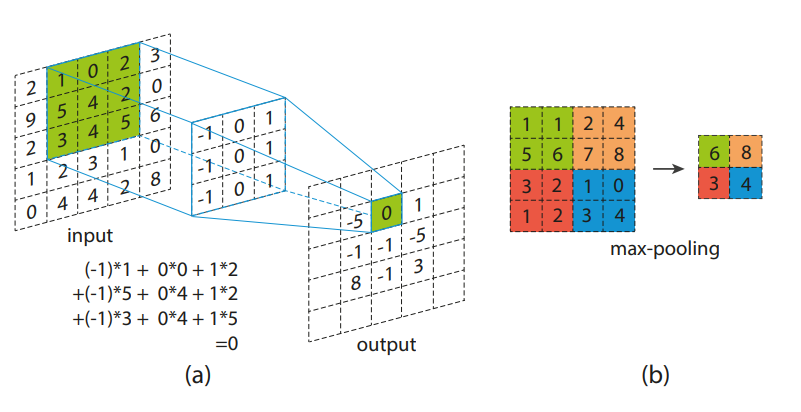
\includegraphics[height=5cm]{./CNN_1.png}
	\end{center}
	\caption{The process of convolution \cite{Liu2016}.}
	\begin{center}
		\label{CNN_1}
	\end{center}
\end{figure}
\FloatBarrier

As a result, the elements of the network  are not densely connected, which allows better generalization and flexibility. This operation in practice allows to extract the important features of the image, such as edges, corners, shapes and many others.  However, unlike in the FC layers, the number of weights is much smaller, which is essential when it comes to high-dimensional images. Following the architecture in Figure \ref{CNN}, the outputs of the convolutional layers are activated with ReLU in a similar manner as in a classical ANN structure. The outputs are then pooled in order to down-sample the image and hence reduce the computational costs \cite{Liu2016}. The commonly used max-pooling operation is shown in Figure \ref{CNN_1} (b). Max-pooling down-samples the image by applying a filter that extracts the maximum value from the region of a feature map. Finally, fully-connected layers complete the structure of the basic CNN. FC layers are used to flatten the outputs from the convolutional layers. In case of the input in Figure \ref{CNN}, this in turn allowed to compute the probability of the input image to represent a number between 0 and 9 \cite{Mahony2019}.

CNNs boosted the performance in computer vision tasks. However, deep learning methods still required extensive training data. Luckily, multiple algorithms emerged as large datasets became available, which were made public as different image classification challenges appeared. The  datasets commonly used in benchmarking are ImageNet \cite{Russakovsky2014}, PASCAL Visual Object Classes(VOC) \cite{Everingham10} and Common Objects in Context(COCO) \cite{Lin2014}. The algorithms that emerged as a result of these challenges will be discussed in the following section. 

\subsection{Image classification}
\label{classification_section} 
It is important to understand the concepts of image classification before moving on to object detection principles. Among the three mentioned earlier, ImageNet was chosen to be a de-facto dataset for running benchmarks.  Different CNN-based models were proposed and some of the most popular models include LeNet \cite{lecun-gradientbased-learning-applied-1998}, AlexNet \cite{NIPS2012_c399862d}, VGGNet \cite{Simonyan2014} and Residual Neural Network(ResNet) \cite{He2015}. As it can be concluded from Figure \ref{image_net}, the classification error dropped lower than the error of the manual detection with the introduction of ResNet, thus approaching the theoretical limits. 

\begin{figure}[htb]
	\begin{center}
		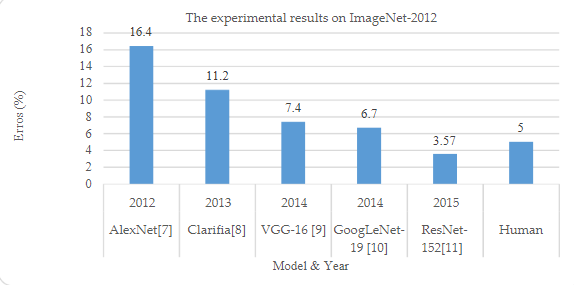
\includegraphics[height=5cm]{./image_net.png}
	\end{center}
	\caption{Evolution of image classifier models evaluated on ImageNet dataset \cite{alom01}.}
	\begin{center}
		\label{image_net}
	\end{center}
\end{figure}
\FloatBarrier

\subsubsection{LeNet}
LeNet architecture (1998) \cite{lecun-gradientbased-learning-applied-1998} is considered to be a pioneer in the field. Its design inherited the classic CNN architecture, but instead it consisted of 7 layers, as presented in Figure \ref{LeNet}. However, the implementation of the paper was not possible for more than 10 years due to limitations in computing power at the time. 

\begin{figure}[htb]
	\begin{center}
		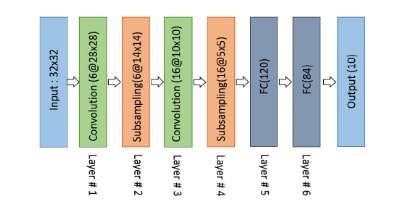
\includegraphics[height=4cm]{./LeNet.png}
	\end{center}
	\caption{LeNet architecture \cite{alom01}.}
	\begin{center}
		\label{LeNet}
	\end{center}
\end{figure}
\FloatBarrier

\subsubsection{AlexNet}
\label{alexnet_section} 
Consequently, AlexNet paper was introduced, which proved the effectiveness of their model, as it outperformed the state-of-the-art implementations and achieved the error rate of 15.3\% \cite{NIPS2012_c399862d}. Figure \ref{AlexNet} displays the proposed network. The architecture of AlexNet is similar to one of LeNet, though it is substantially deeper and has more than 60 million adjustable parameters. It has 5 convolutional layers of varying kernel size. The convolutional layers are followed byt ReLU activation functions and max-pooling layers. The architecture is finalized by attaching two FC layers with dropout rate of 0.5 and one softmax layer.

During dropout, there is a probability that the neuron will be excluded from computations in the subsequent layer. Utilizing such technique proved to be essential to fight over-fitting in FC layers and improve generalization  \cite{JMLR:v15:srivastava14a}. 

AlexNet architecture was the first CNN to split the model into two parts and to leverage mulitple GPUs in training due to GPU memory limitations of 3GB at the time \cite{NIPS2012_c399862d}. 

\begin{figure}[htb]
	\begin{center}
		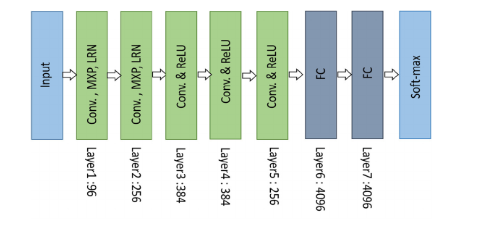
\includegraphics[height=4cm]{./AlexNet.png}
	\end{center}
	\caption{AlexNet architecture \cite{alom01}.}
	\begin{center}
		\label{AlexNet}
	\end{center}
\end{figure}
\FloatBarrier

\subsubsection{VGG}
Another milestone was achieved with the discovery proposed in VGGNet \cite{Simonyan2014}. This work proved that the depth of the network produces a significant impact on the performance of the CNN in classification tasks \cite{alom01}. Three different versions of the model were proposed with 11, 16 and 19 layers, respectively and with the deeper model being the best in performance, but more expensive in terms of computation. Equivalently to AlexNet, the network has blocks of convolutional layers of a mixed kernel size, followed by a ReLU block and max-pooling. The network is finalized with three FC and one softmax layers. 

\begin{figure}[htb]
	\begin{center}
		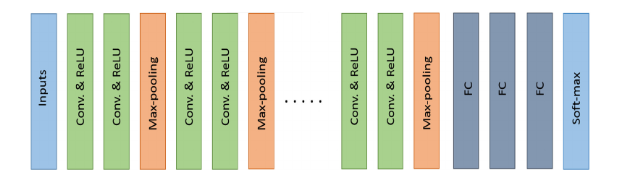
\includegraphics[height=4cm]{./vgg.png}
	\end{center}
	\caption{VGG architecture \cite{alom01}.}
	\begin{center}
		\label{VGG}
	\end{center}
\end{figure}
\FloatBarrier

\subsubsection{ResNet}
ResNet architecture \cite{He2015}, which was proposed in 2015, discovered that after reaching certain depth of the network, the performance of the model degrades. He et al. \cite{He2015} suggested that this happens due to the "vanishing gradient" problem. As the model gets deeper, several applications of the chain rule on during backpropogation tend to diminish either all the way to zero or becomes too large. As a result, no update is applied on the weights and hence, no training takes place. He et al. proposed to utilize a residual block, illustrated in Figure \ref{resnet}, which is used to skip some of the layers in between.  This solution essentially mitigates the problem of vanishing gradients by allowing the training loop to skip parts of the network that negatively affect the performance.

\begin{figure}[htb]
	\begin{center}
		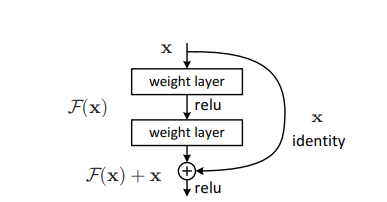
\includegraphics[height=4cm]{./resnet.png}
	\end{center}
	\caption{Residual block of ResNet \cite{He2015}.}
	\begin{center}
		\label{resnet}
	\end{center}
\end{figure}
\FloatBarrier

ResNet adopts the VGG-19 architecture, but adds a skip connection block. He et al. implemented multiple versions of the model and the largest one is 152 layers deep. Nonetheless, the network has less trainable parameters than VGG, which substantially improves the training speed while preserving accuracy due to the residual block. As a result, the proposed model achieved the error of 3.57\% on ImageNet dataset, which is lower than the human eye error \cite{He2015}.

\begin{figure}[htb]
	\begin{center}
		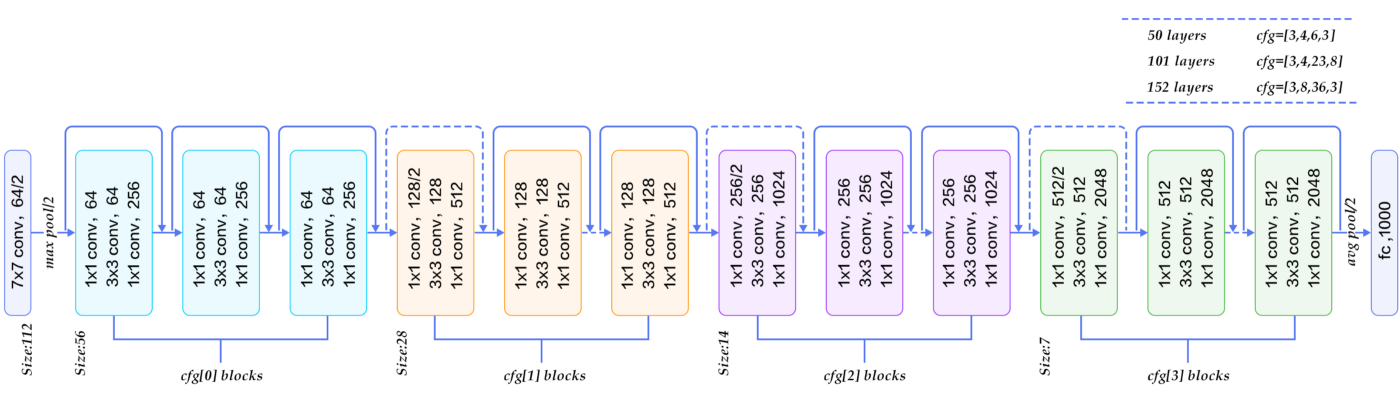
\includegraphics[width=16cm]{./resnetFull.png}
	\end{center}
	\caption{ResNet architecture \cite{resnet50}.}
	\begin{center}
		\label{resnetFull}
	\end{center}
\end{figure}
\FloatBarrier


%Often, image processing tasks are classified into three main learning paradigms - supervised,  %unsupervised and semi-supervised learning.


\subsection{Object detection}
\label{obj_detection_section} 
The problem of object detection is an extended version of the image classification problem. However, unlike image classification, object detection aims to recognize not only the object, but also to localize it. Prior to arrival of deep learning, object detection considered to be a difficult task. With the discovery of the CNN architecture, the traditional computer vision techniques became obsolete. Since then, multiple different detector algorithms emerged. A typical object detection network contains two important modules - the base (or backbone) network  and the detector network. A base network is usually one of the pre-trained VGG or ResNet models, presented in the previous chapter. A base network acts as a feature extractor, and the features are then passed to a detector. Generally speaking, deep learning based detector networks can be classified into two categories: single- and two-stage detectors \cite{Zaidi2021}, as shown in Figure \ref{OD}.  

\begin{figure}[htb]
	\begin{center}
		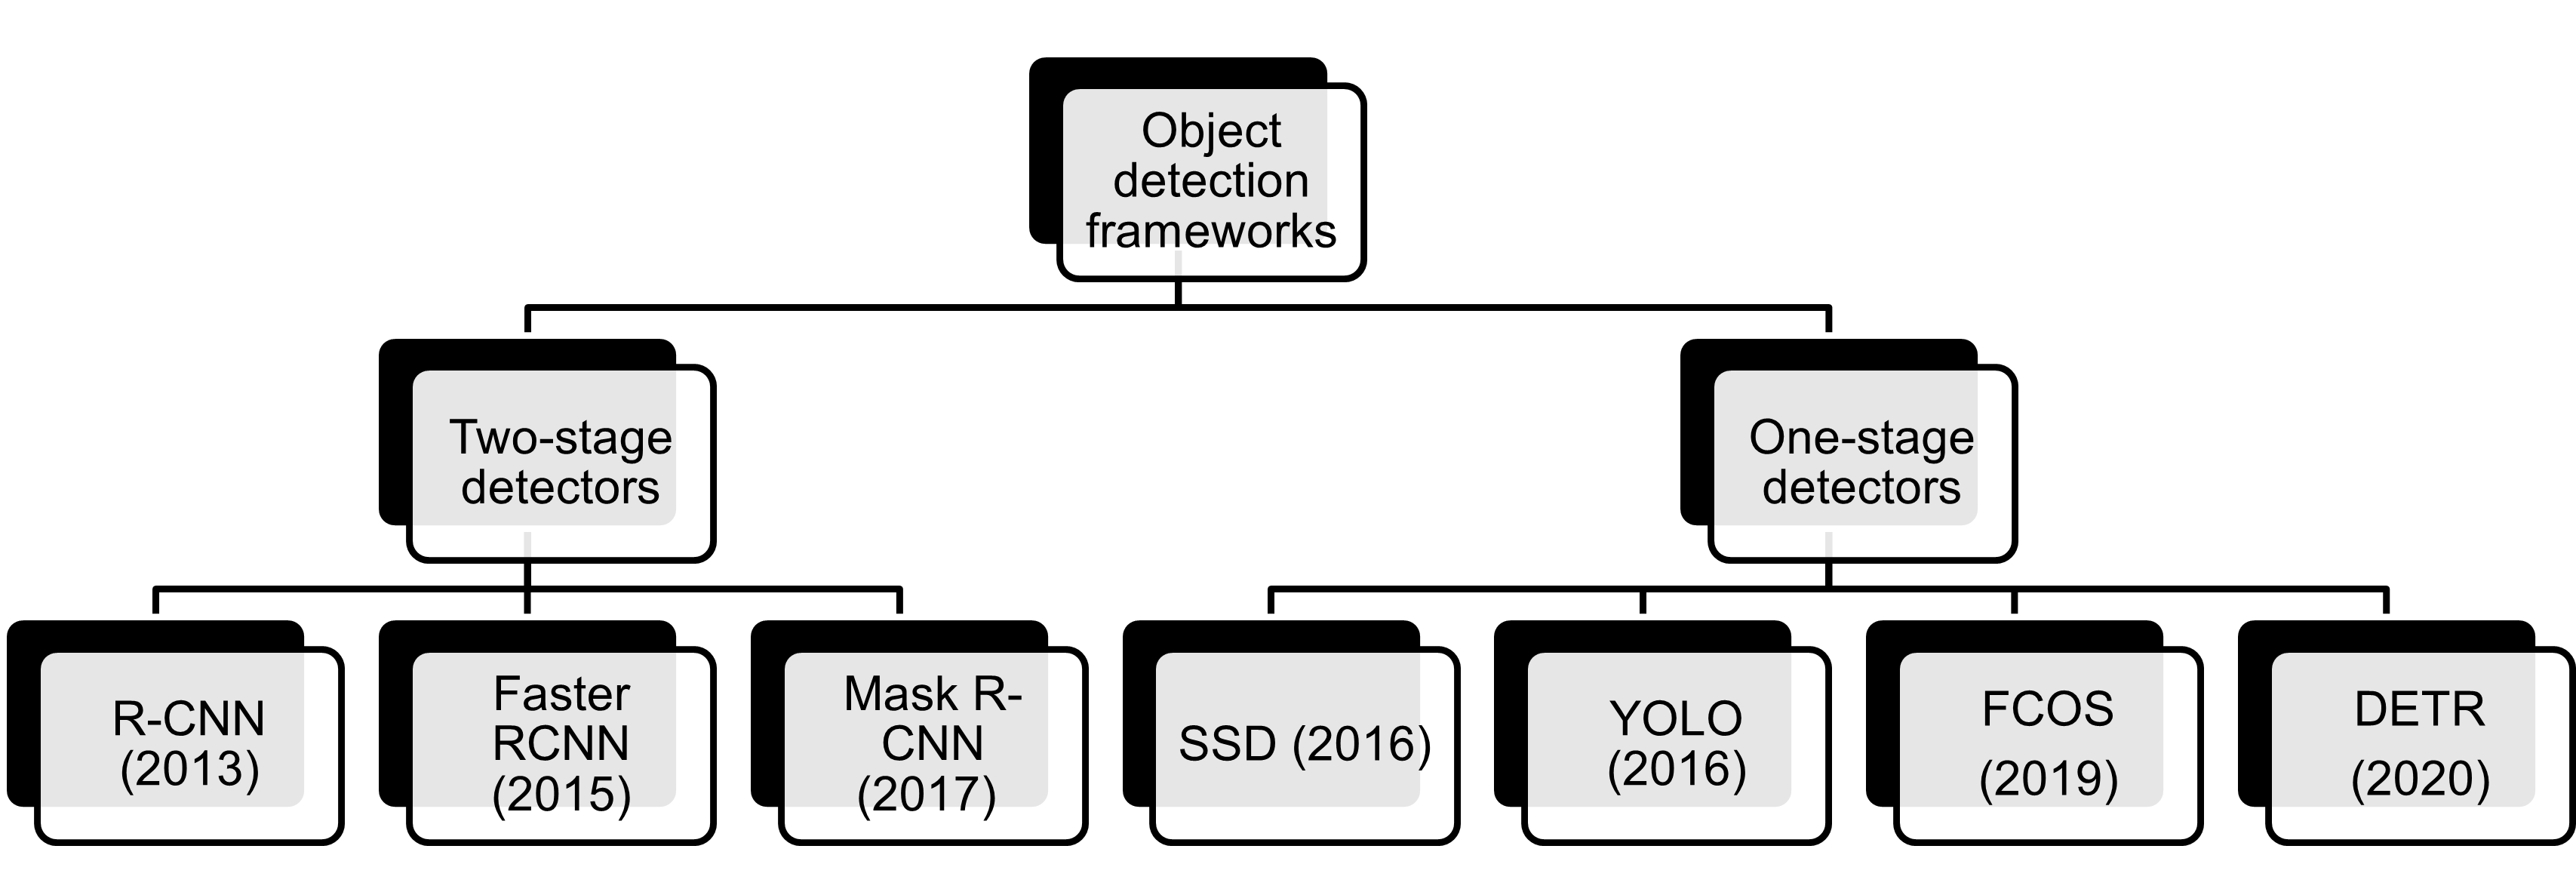
\includegraphics[width=16cm]{./OD.png}
	\end{center}
	\caption{Types of object detectors.}
	\begin{center}
		\label{OD}
	\end{center}
\end{figure}
\FloatBarrier

Two-stage object detectors attempt to propose regions of the image that contain an object first, and then run the task of classification and localization on the proposed region. On the other hand, single-stage detectors try to detect objects directly without running the  Region Proposal Network (RPN). Figure \ref{fig:1vs2stage} illustrates the key differences in the architecture.

\begin{figure}[htb]
    \centering
    \subfloat{\raisebox{0.13\height}{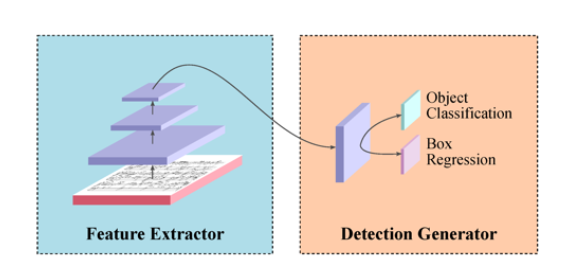
\includegraphics[width=6cm]{./1stage.png} }}%
    \qquad
    \subfloat{{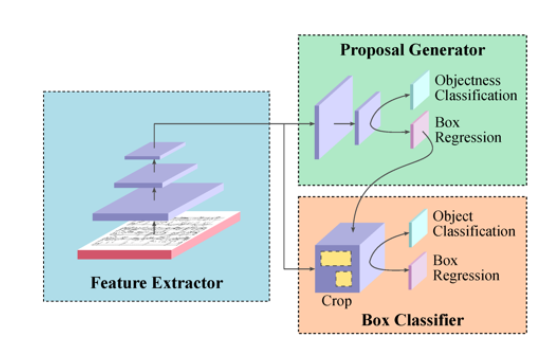
\includegraphics[width=6cm]{./2stage.png} }}%
    \caption{A simple single-stage detector(left) compared to a two-stage detector(right) \cite{app8091488}.}\label{fig:1vs2stage}%
\end{figure}
\FloatBarrier

Typical examples of the single-stage networks are RetinaNet \cite{Lin2017}, Single-shot detector(SSD) \cite{Liu2015} and You Only Look Once(YOLO) \cite{Redmon2015a}. In two-stage detectors, Region-based CNN(R-CNN) \cite{Girshick2013}, Fast-RCNN \cite{Girshick2015} and Faster-RCNN \cite{ima} are considered to be the most important discoveries. Figure \ref{OD} also mentions detectors such as FCOS \cite{Tian2019}, Mask-RCNN \cite{He2017} and DETR \cite{Carion2020}. Although they show competitive performance, they are not reviewed in the thesis as they are not relevant to the method introduced in the \nameref{Methodology}.  The following subsection will introduce the reader to some of the main concepts of the selected detectors. 


\subsubsection{R-CNN}

Figure \ref{rcnn} shows the structure of the R-CNN network \cite{Girshick2013}. R-CNN has been one of the first CNN-based models to be introduced \cite{Zaidi2021}. Girshick et al. essentially suggested to use a module that extracts the object proposals and then to pass it to a CNN. The CNN would then extract the features relevant, which would in turn allow to classify the proposed region as well as to localize it. In their original experiments, the selective search algorithm  \cite{Uijlings13} was used to produce roughly 2000 regions. AlexNet  \cite{NIPS2012_c399862d} was used as a backbone CNN to extract vectors of 4096 size dimensions. The features were then passed to binary classifiers that are bound to a certain class. As multiple regions are returned, non-maximum suppression(NMS) \cite{Hosang2017}  is used to identify the best proposal for the object. 

Unfortunately, the inference process in R-CNN took a whole 47 seconds per image \cite{Girshick2013}, which was not fast enough to be remain relevant in the object detection field. 

\begin{figure}[htb]
	\begin{center}
		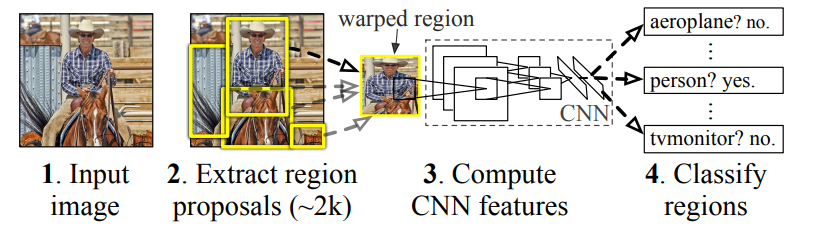
\includegraphics[width=12cm]{./rcnn.png}
	\end{center}
	\caption{R-CNN overview \cite{Girshick2013}.}
	\begin{center}
		\label{rcnn}
	\end{center}
\end{figure}


\subsubsection{Fast-RCNN}
Unlike the classic R-CNN system, where the components such as the classifier and the regressor have to be trained separately, the same authors of the RCNN  model also introduced a Fast-RCNN model \cite{Girshick2015}, which proposed an end-to-end trainable system. Additionally, the region-of-interest(ROI) pooling layer was proposed. This ROI component essentially divides the image into a grid of a fixed size and applies average pooling. The resulted one-level pyramid of the image is used as a feature map for the detector head. This allows the rest of the network to focus purely on the features extracted for the proposed regions. Finally, two additional FC output layers are appended, where the first one classifies the features by returning the probability of N object classes in range $(0, N+1]$, which includes the background class as well. The other one returns a vector of a size $(0, 4\times N]$, thus including the bounding box coordinates for the foreground classes only \cite{Girshick2015}. Fast-RCNN showed a significant($\times 146$) speed improvement as compared to the R-CNN, thus allowing it to be used in real-time applications \cite{Girshick2013}. The original architecture of Fast-RCNN is shown in Figure \ref{fast_rcnn} below. 

\begin{figure}[htb]
	\begin{center}
		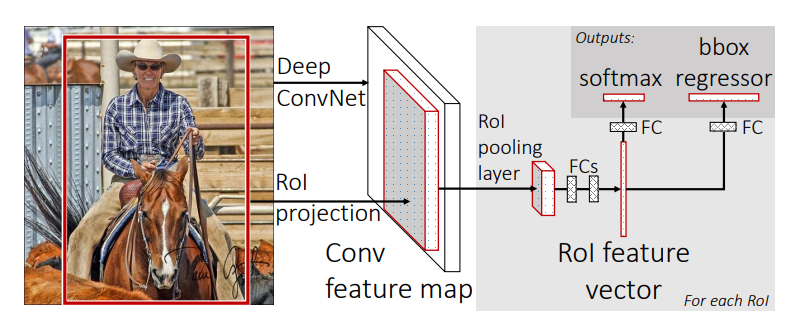
\includegraphics[width=10cm]{./fast_rcnn.png}
	\end{center}
	\caption{Fast-RCNN overview \cite{Girshick2015}.}\label{fast_rcnn}
	\begin{center}
	\end{center}
\end{figure}
\FloatBarrier

\subsubsection{Faster-RCNN} 
Ren et al. \cite{ima} discovered that even though Fast-RCNN was significantly faster than the preceding networks, the region proposing process was still causing a bottleneck. Therefore, in the novel Faster-RCNN \cite{ima} architecture it was suggested to replace the legacy region proposal module with a fully-convoluted architecture called region proposal network(RPN) \cite{Girshick2013}. Instead of using the one-level image pyramid to solve the problem as it was proposed by Girshick et al. \cite{Girshick2015}, Faster-RCNN utilizes anchor boxes of different aspect ratios to propose object candidates. Similarly to any other CNN, the features in Faster-RCNN are extracted from the convolutional layers based on a VGG backbone. The features maps are then sent to the RPN, which in practice is a sliding window  of $n\times n$ $(n=3)$ dimensions. At every sliding window position, the $k$ number of object proposals are predicted. Such boxes are called "anchors" as illustrated in Figure \ref{fig:faster_rcnn}. The acquired $2k$ classification predictions whether the proposed region is an object of interest or not and $4$ regression outputs of the bounding box coordinates are then mapped back to the ROI layer and, eventually, to the FC layers that predict the class of the proposed object \cite{ima}. 


\begin{figure}[htb]
    \centering
    \subfloat{{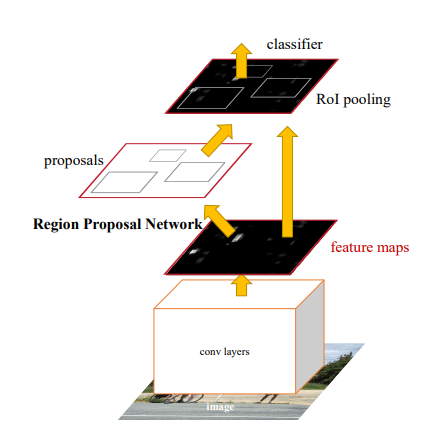
\includegraphics[width=6cm]{./faster_rcnn.png} }}%
    \qquad
    \subfloat{\raisebox{0.5\height}{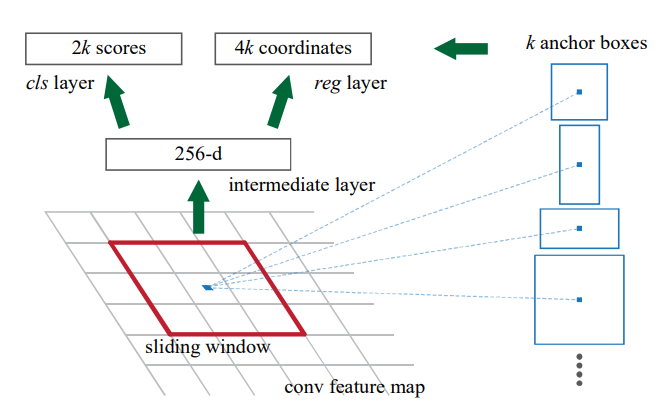
\includegraphics[width=6cm]{./faster_rcnn_rpn.png} }}%
    \caption{Faster-RCNN overview and its RPN module \cite{ima}.}
    \label{fig:faster_rcnn}%
\end{figure}
\FloatBarrier

As the network returns the predictions, the loss function is calculated as in Equation \ref{faster_rcnn_loss}:  
\begin{equation}
\begin{array}{r}
L\left(\left\{p_{i}\right\},\left\{t_{i}\right\}\right)=\frac{1}{N_{c l s}} \sum_{i} L_{c l s}\left(p_{i}, p_{i}^{*}\right) \\
+\lambda \frac{1}{N_{\text {reg }}} \sum_{i} p_{i}^{*} L_{r e g}\left(t_{i}, t_{i}^{*}\right)
\end{array}
\label{faster_rcnn_loss} 
\cite{ima},
\end{equation}

where $p_i$ is a probability of the predicted anchor $i$ to be an object,  $p_{i}^{*}$ is a ground-truth label from 0 to 1, $t_i$ is a vector with 4 coordinates of the bounding box and $t_{i}^{*}$ is its corresponding ground-truth vector. $\lambda$ is a trade-off between the $L_{cls}$ and $L_{reg}$, where $L_{c l s}$ is calculated as a binary log loss and $L_{reg}$ uses a smooth $L_1$ loss that was introduced in Fast-RCNN \cite{Girshick2015}.  




This implementation, unlike Fast-RCNN, allowed to return predictions nearly in real time with the breakthrough of 5 frames per second(FPS) \cite{ima}.
Although the two-stage Faster-RCNN detector is nearly 7 years old at the time of writing this thesis, it is still one of the most widely used detectors in the field, as can be noticed from Figure \ref{popularity}. In later chapters, this work will focus on the Faster-RCNN implementation. Nevertheless, it is worth mentioning single-stage competitors. Often they are slightly weaker in terms of accuracy, compared to two-stage detectors. However, these detectors offer a significant improvement in robustness as compared even to the fastest one of the two-stage detectors, Faster-RCNN. 

\begin{figure}[htb]
	\begin{center}
		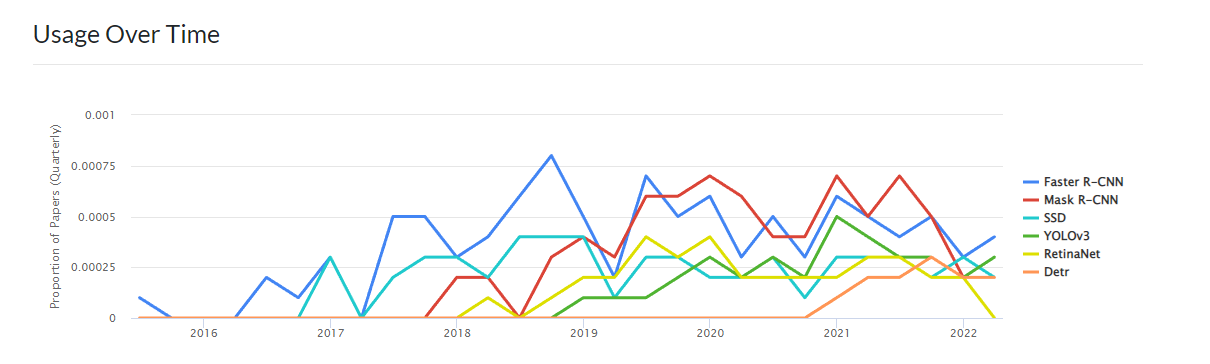
\includegraphics[width=14cm]{./detectorsPopularity.png}
	\end{center}
	\caption{The popularity of different detectors according to  \cite{paperswithcode_1:2022}.}
	\begin{center}
		\label{popularity}
	\end{center}
\end{figure}
\FloatBarrier


\subsubsection{YOLO}
\label{yolo_section} 

Unlike the two-stage methods presented, You Only Look Once(YOLO) \cite{Redmon2015a} algorithm attempts to solve the object detection problem purely as a regression problem by predicting the bounding boxes of the objects directly without region proposals. The YOLO network instead splits the image into a grid of $S\times S$ cells, for which a $B$ number of bounding boxes and $C$ probabilities of the class and  are predicted \cite{Redmon2015a}. The overview of the detection process is shown in Figure \ref{yolo}. The principle of the YOLO grid component is broadly similar the one of R-CNN \cite{Girshick2013}, where the algorithm of selective search \cite{Uijlings13} is used to propose regions. However, instead of proposing more than 2000 regions, YOLO only returns 98 proposal boxes per image. This, along with having an optimized single-stage detection process, allowed YOLO to achieve impressive nearly real-time FPS results. Redmon et al. reported YOLO to sustain the average FPS of 45, while the most accurate version of the Faster-RCNN network had 7 FPS \cite{Redmon2015a}. However, the proposed network still has multiple limitations, which were addressed in later iterations of the paper  \cite{Redmon2016, Redmon2018a}.

The architecture consists of 24 cascaded convolutional and 2 FC layers. The convolutional layers are first pre-trained on the ImageNet dataset \cite{Russakovsky2014}. The image size is reduced by applying $1\times1$ convolutional layers in between, also referred to as "reduction layers"  \cite{Redmon2015a}. The simplified architecture is presented in Figure \ref{ssd}.

\begin{figure}[htb]
	\begin{center}
		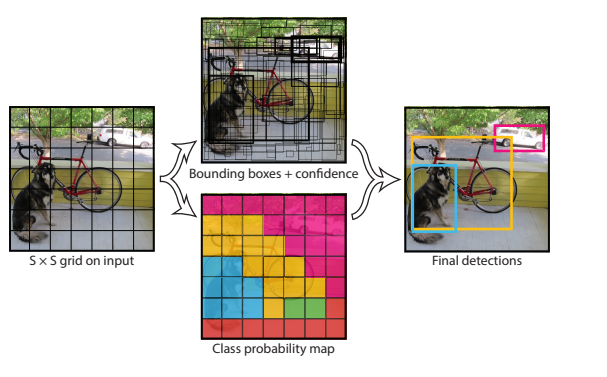
\includegraphics[width=12cm]{./yolo.png}
	\end{center}
	\caption{YOLO overview \cite{Redmon2015a}.}
	\begin{center}
		\label{yolo}
	\end{center}
\end{figure}
\FloatBarrier


%%\subsubsection{RetinaNet}

%%\begin{figure}[htb]
%%	\begin{center}
%%		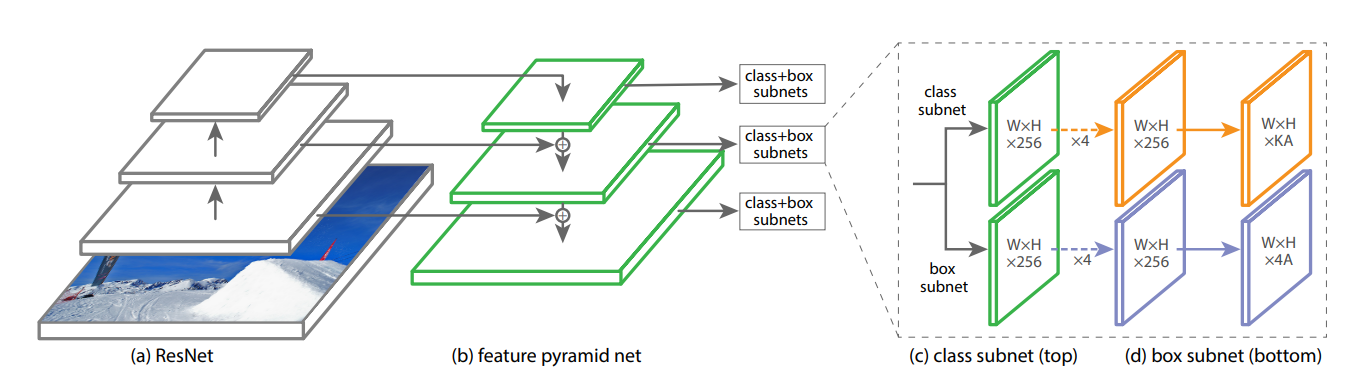
\includegraphics[width=14cm]{./retinaNet.png}
%%	\end{center}
%%	\caption{RetinaNet overview\cite{Lin2017}}
%%	\begin{center}
%%		\label{retinanet}
%%	\end{center}
%%\end{figure}
%%\FloatBarrier


\subsubsection{SSD}
Another implementation of a single-stage network worth mentioning is a Single-Shot MultiBox detector(SSD) \cite{Liu2015}. The differences in architectures of SSD and YOLO are displayed in Figure \ref{ssd}. Liu et al. proposed a model that detects objects in real-time while preserving the accuracy. First, the image is fed into the backbone CNN, in the original experiments - VGG-16. The SSD head layers added after the backbone network are convolutional as well. Similarly to YOLO, the image is split into a grid of $n\times n$ size, where it benefits from the anchor boxes of varying aspect ratio. 


\begin{figure}[htb]
	\begin{center}
		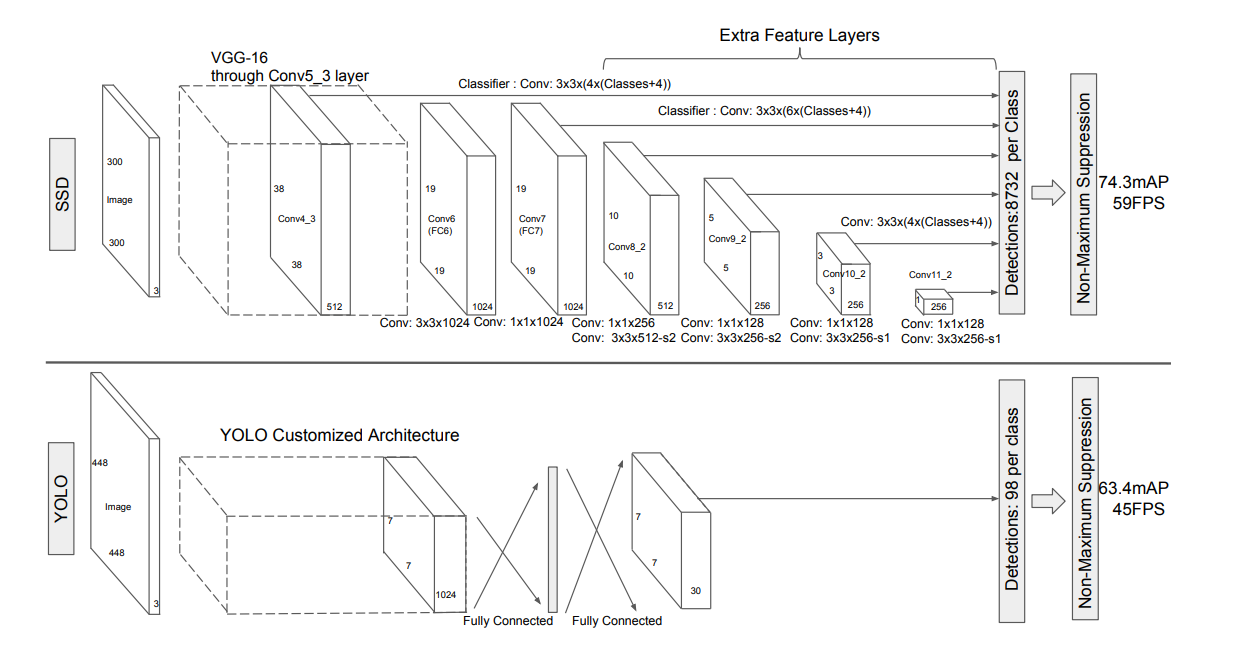
\includegraphics[width=14cm]{./ssd_yolo.png}
	\end{center}
	\caption{SSD compared to YOLO \cite{Liu2015}.}
	\begin{center}
		\label{ssd}
	\end{center}
\end{figure}
\FloatBarrier

However, as the objects might not always be within the grid boundaries, as can be noticed from Figure \ref{ssd_boxes}. Therefore, SSD paper introduced a concept of anchor boxes with offsets. The anchor boxes with offsets that have the highest overlap with the ground truth box of the object are then passed to FC layers to predict the class and the location of the object. 

\begin{figure}[htb]
	\begin{center}
		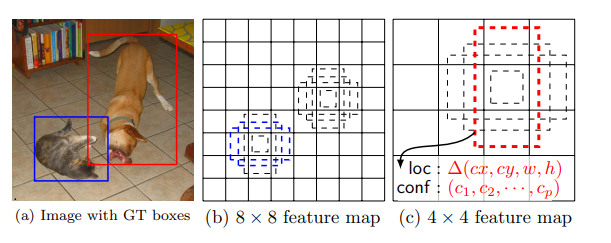
\includegraphics[width=12cm]{./ssd_boxes.png}
	\end{center}
	\caption{SSD anchor boxes \cite{Liu2015}.}
	\begin{center}
		\label{ssd_boxes}
	\end{center}
\end{figure}
\FloatBarrier

The key object detection models of the last decade are presented in Table \ref{detectorsTable} below. As it can be deducted from the table, Faster-RCNN shows the best performance on the PASCAL VOC dataset, while YOLO demonstrated the highest FPS. The survey of Zaidi et al. \cite{Zaidi2021} also discusses lightweight models. However, for the purpose of this study, the detection accuracy is the primary focus rather than speed, thus their review will be omitted. 

\begin{table}[htb]
	\captionof{table}{Overview of object detectors \cite{Zaidi2021}. }
	\begin{center}
		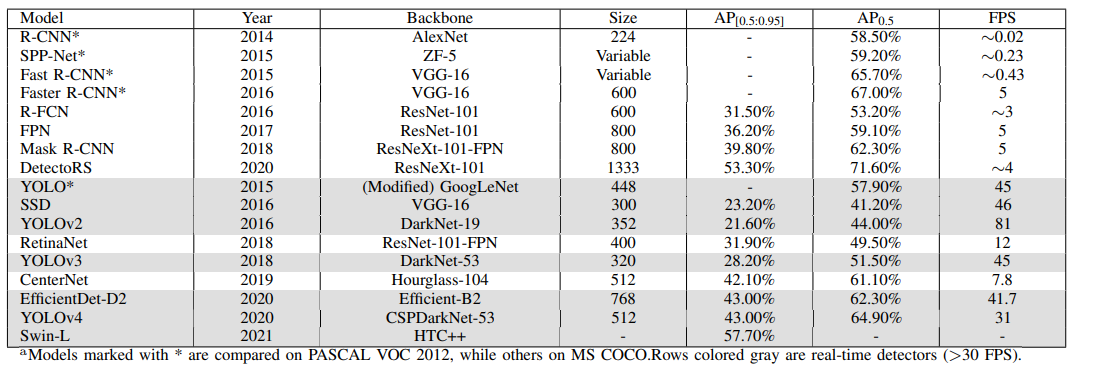
\includegraphics[width=16cm]{./detectorsTable.png}
	\end{center}
	\begin{center}
		\label{detectorsTable}
	\end{center}
\end{table}
\FloatBarrier

As it can be seen from Table \ref{detectorsTable}, there are multiple models that are not covered in this section. Additionally, there are several detectors that show promising results in the domain-adaptive object detection setup, such as FCOS \cite{Tian2019} and DETR \cite{Zhang2021b}. However, as their performance is not yet extensively evaluated, they will be omitted from this thesis. 

\subsection{Object detection in industrial environments}
Although object detection is an extremely diverse field with applications varying from medicine \cite{9689485} to self-driving vehicles \cite{Janai2017, Shan2018}, the industrial object detection is mostly limited to safety and process monitoring \cite{Awalgaonkar2020, Banf2022}. Fewer research has addressed the topic of industrial object detection. In general, many of the introduced object detection methods can be applied to this problem directly as it is. Malburg et al. \cite{MALBURG2021581} has evaluated multiple different versions of object detection models such as YOLO \cite{Redmon2015a} in an industrial setup. However, often in industrial environments severe challenges such as overlapping and occlusion take place. Moreover, the object instances often are represented in multiple scales. Therefore, it is often impossible to obtain reliable results using a standard object detector architecture. Wu et al. \cite{Wu2022} has recently addressed the problem of industrial object detection using an R-CNN based approach that leverages Feature Pyramid Networks to improve detection at multiple scales and NMS with penalty factors to eliminate occlusion problem. However, the proposed method does not consider the data availability limitations and confidentiality issues that were outlined in the \nameref{objective}. On the other hand, Kim et al. \cite{Kim2020} minimized the need for labeling from a human by utilizing a deep active learning model. While the core of this approach is a standard Faster-RCNN \cite{ima} network, Kim et al. also proposed to utilize uncertainty evaluation in order to enable the model to label images interactively over time. As the training advances, the model evaluates whether the predicted bounding boxes are reliable or not using the sum of entropy for each bounding box. In the subsequent stage the model requests the user to manually label 10\% of the data with highest uncertainty. The model is then retrained with the updated knowledge. Although this approach seems promising, it  does not consider the domain shift phenomenon that takes place in the setup defined by the \nameref{objective}. Later sections of the thesis will address this phenomenon. 

\todo{Write more about this active learning method if there is time} 


\subsection{Transfer learning}
\label{transferLearning} 
In this section, the multiple transfer learning(TL) techniques will be introduced. Despite the fact that the methods discussed in previous chapters have been successfully implemented in various scenarios, ML in general often struggles to apply such methods in real life. This is normally caused by insufficient training data, as it is often expensive to collect it, both in terms of time, financially, and sometimes simply not possible at all due to data accessibility issues \cite{Zhuang2019}. Moreover, the requirement of having to train the models on new massive datasets often make ML solutions inefficient in practice. For this reason, TL concepts have been found advantageous as it addresses transferring knowledge learned from one task, domain or distribution to another. Here and in the subsequent sections, the notations are identical to those outlined by Pan et al. \cite{Pan2010} and are introduced as follows:  

\todo{mention later: Zhuang2019: TL does not always bring benefit}

\begin{itemize}
\item A domain $\mathcal{D}$ can be defined as a composite term, which is characterized by two elements: feature space $\mathcal{X}$ and a marginal probability distribution $P(X)$; $X=\left\{x_{1}, \ldots, x_{n}\right\} \in \mathcal{X}$. With this being said, two domains are defined as different if their feature spaces or marginal probability distributions are different. In this thesis, the domains are restricted with one source $\mathcal{D_S}$ and one target $\mathcal{D_T}$ domains \cite{Pan2010}. 
\item Similarly, a task $\mathcal{T}$ can be defined by its label space $\mathcal{Y}$ and a conditional probability of $\mathcal{Y}$ given $X$, e.g. $P(Y \mid X)$, $Y=\left\{y_{1}, \ldots, y_{n}\right\} \in \mathcal{Y}$. In practice, a conditional probability is defined as a function that can learn to predict a label $y_i$ given a sample vector $x_i$ \cite{Pan2010}. 
\end{itemize} 


 
\begin{figure}[htb]
	\begin{center}
		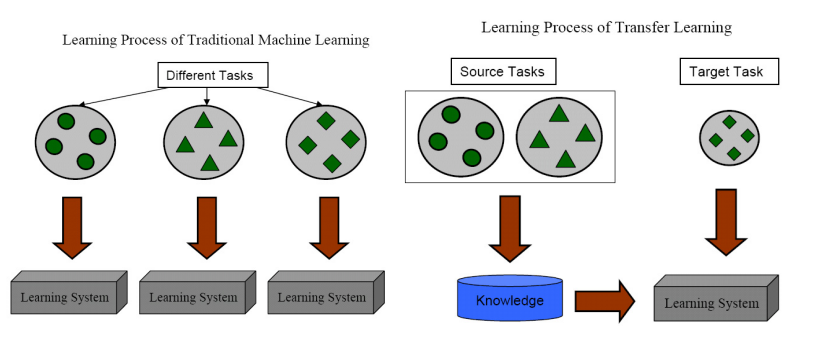
\includegraphics[width=16cm]{./TL.png}
	\end{center}
	\caption{Comparison of ML to TL \cite{Pan2010}.}
	\begin{center}
		\label{TL}
	\end{center}
\end{figure}
\FloatBarrier

Sun et al. \cite{SUN201584} describes TL as a method to transfer knowledge when the feature space between the two given source and target domains is different, meaning that $\mathcal{X}_{S} \neq \mathcal{X}_{T}$. Pan et al. \cite{Pan2010} mentions that transfer learning can be also defined when the marginal probability is different, meaning that $P_{S}(X) \neq P_{T}(X)$. Similarly, transfer learning can be applied when $\mathcal{T}_{S} \neq \mathcal{T}_{T}$. An example of a simple TL problem is training a model that was trained for classifying cats, but instead is  required to learn a new task such as classifying dogs. However, in various scenarios, the task is essentially the same but the domain is similar yet different. For instance, a model that was trained to identify cats in sketches, is instead required to identify cats in real images. Solving such tasks is the main focus of domain adaptation(DA). Often the terms "domain adaptation" and "transfer learning" are used interchangeably. However, according to Wang et al. \cite{Wang2018} and Zhang et al. \cite{Zhang2021}, domain adaptation(DA) is a special case of TL. In scientific terms, the problem that DA attempts to solve can be defined when the source and target feature spaces are the same $\mathcal{X}_{S}=\mathcal{X}_{T}$, but the marginal probability distribution is not $P\left(\mathcal{X}_{S}\right) \neq P\left(\mathcal{X}_{T}\right)$ \cite{SUN201584}. This is not to be confused with semi-supervised machine learning, where both labeled and unlabeled data is typically supplied from one domain \cite{SUN201584}. 

%https://www.v7labs.com/blog/transfer-learning-guide


\subsubsection{Domain adaptation}
\label{DA_section} 
Domain Adaptation (DA) has lately been gaining popularity in both image classification and object detection tasks \cite{Zhang2021}. Typically, DA is used to predict a label given the data from a source domain and limited or no data from the target domain. Most importantly, DA addresses the domain shift problem \cite{Zhang2021}. In a DA problem, a domain shift, also known as a distributional shift or dataset bias, can be defined as a change in distribution of data between source and target domains. 


Zhang et al. \cite{Zhang2021} classify DA methods into three categories that are similar to ML types - supervised, semi-supervised, and unsupervised DA. Alternatively, Oza et al. \cite{Oza2021} classify the collected DA methods into semi-supervised, weakly-supervised and unsupervised DA. Indeed, supervised DA is not commonly used since the primary goal of DA is to reduce the domain shift when the data availability is limited. 

According to Zhang et al. \cite{Zhang2021}, different methods that attempt to solve the distribution shift problem by minimizing the distance between marginal, conditional or joint distributions. 

The visual representation of these distribution alignment types are shown in Figure \ref{distribution} and the methods in the following subsections attempt to minimize the domain shift by one way or another. 

\begin{figure}[htb]
	\begin{center}
		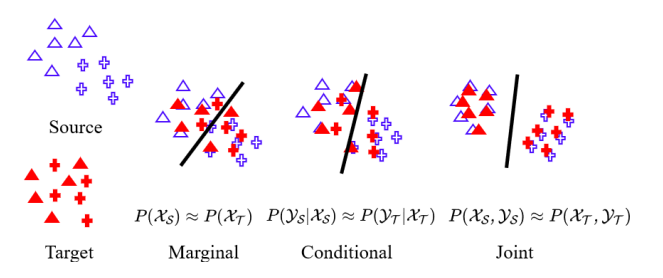
\includegraphics[width=12cm]{./distribution.png}
	\end{center}
	\caption{Distribution alignment types \cite{Zhang2021}.}
	\begin{center}
		\label{distribution}
	\end{center}
\end{figure}
\FloatBarrier 



\subsection{Domain adaptive object detection}
\label{DAobj} 
Next subsection will discuss some of the methods that were proposed at different times to solve the problem of domain shift in object detectors. Oza et al.  \cite{Oza2021} have extensively reviewed and grouped the existing approaches into following six categories:
\begin{enumerate}
	\item Adversarial feature learning
	\item Pseudo-label based self-training
	\item Image-to-image translation
	\item Domain randomization 
	\item Mean-teacher training
	\item Graph reasoning
\end{enumerate} 

Many of the methods collected by Oza et al. overlap with each other and fall into more than one group. In this thesis, a few methods will be briefly reviewed for each of the categories above. Some of the methods are listed in Figure \ref{UDA_OD}.

\begin{figure}[htb]
	\begin{center}
		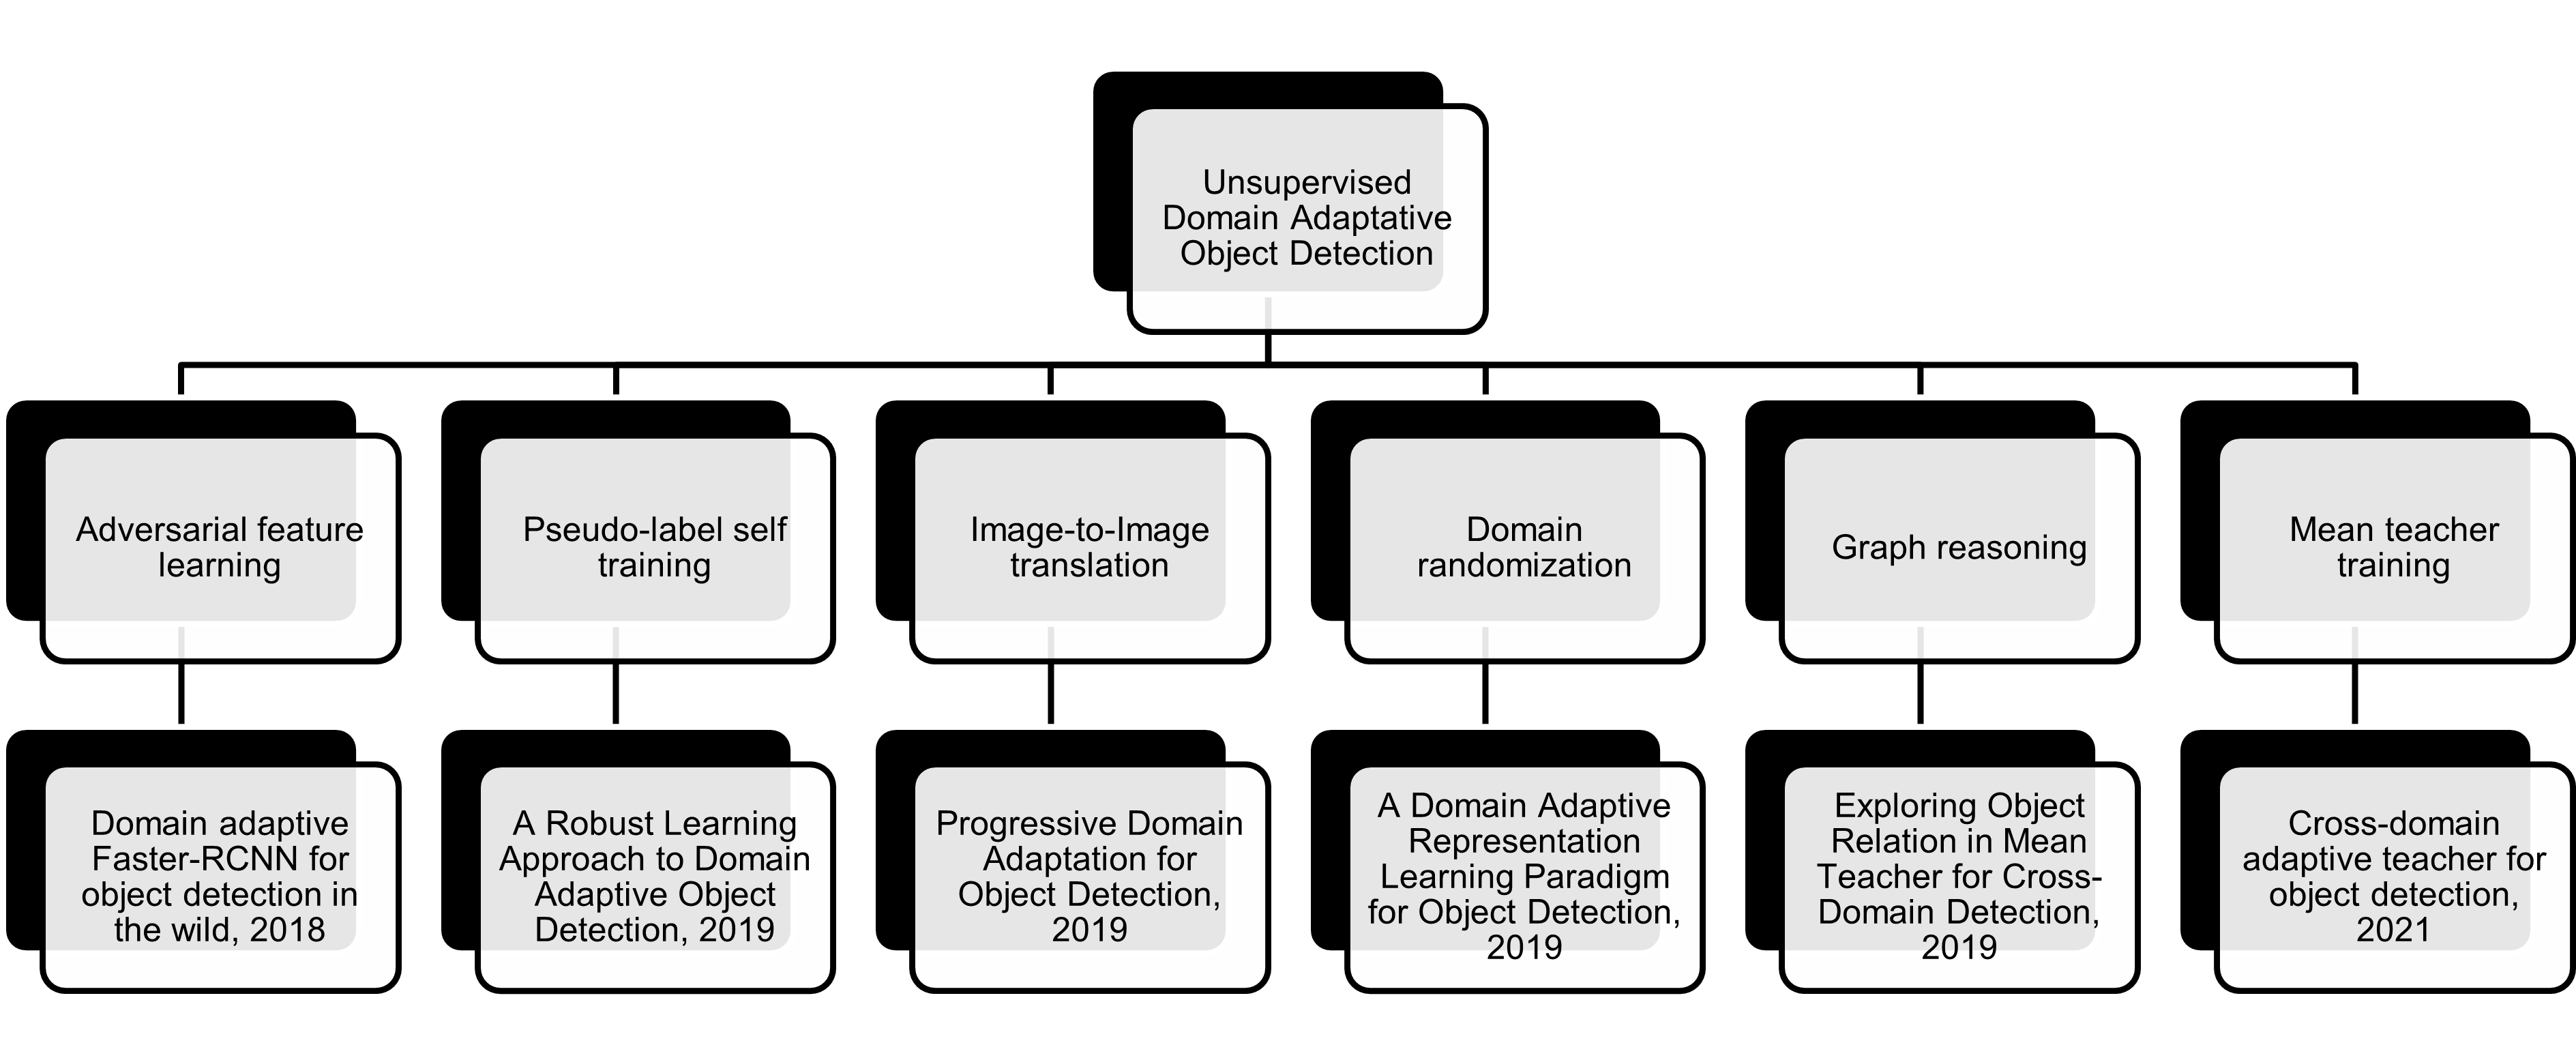
\includegraphics[width=16cm]{./UDA_OD.png}
	\end{center}
	\caption{Unsupervised Domain Adaptive Object Detection.}
	\begin{center}
		\label{UDA_OD}
	\end{center}
\end{figure}
\FloatBarrier

In the following methods, it will be assumed that $\mathcal{D_S}$ and $\mathcal{D_T}$ originate from similar yet different distributions. Additionally, the papers introduced in the following section address unsupervised domain adaptation(UDA) problem, which is naturally more sophisticated than a supervised DA.

\subsubsection{Gradient reversal layer}

One of the key components in a typical domain adaptive setup for both image classification and object detection problems is a gradient reversal layer(GRL) that has been proposed by Ganin et al. \cite{Ganin2015}. The authors suggest that in order to successfully solve the domain adaptation problem, the prediction should be based on the features that cannot differentiate between the source and target domains. In other words, the network should propose features that are common for both domains. Figure \ref{DANN} illustrates the Domain-Adversarial Neural Network (DANN) proposed by Ganin et al. \cite{Ganin2015}. 

\begin{figure}[htb]
	\begin{center}
		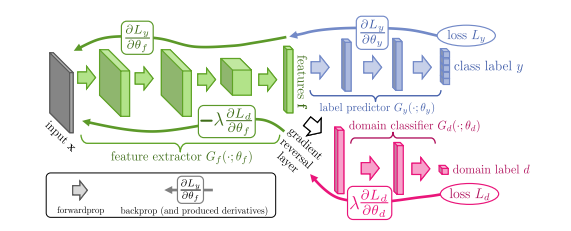
\includegraphics[width=16cm]{./GRL.png}
	\end{center}
	\caption{Domain-adversarial neural network and GRL \cite{Ganin2015}.}
	\begin{center}
		\label{DANN}
	\end{center}
\end{figure}
\FloatBarrier

The network is essentially a simple feed-forward network with a feature extractor and a predictor that classifies the input. Two additional components are appended to the last layer of the feature extractor - a gradient reversal layer(GRL) and a domain classifier. On the forward pass of the DANN, the network attempts to predict the class and the domain labels and GRL acts as an identity function. During the backpropogation, the GRL multiplies the gradient of the domain classifier by a fixed negative weight constant $\lambda$. This enables the domain classier to maximize the domain classification loss and, therefore, "confuse" the feature extractor and force it to generate only domain invariant features \cite{Ganin2015}. 
\todo{Perhaps add more math about GRL} 


\subsubsection{Adversarial feature learning}
\label{adv_approach} 

Although DANN implementation is originally meant for domain adaptive image classification, GRL is a fundamental component in adversarial feature learning of object detectors and will be referenced in the subsequent sections of the thesis. 

The majority of the methods, collected in the survey by Oza et al. \cite{Oza2021}, are based on the two-stage object detectors and Faster-RCNN \cite{ima} in particular. This has been presumably facilitated by Pytorch \cite{NEURIPS2019_9015} package in Python and frameworks such as Detectron \cite{Detectron2018} and Detectron2 \cite{wu2019Detectron2} that enabled researchers to extend the possibilities of Faster-RCNN and improve its scalability. With the arrival of the mentioned tools and their pre-trained models, Faster-RCNN became a good starting point to experiment with new tasks, which was done by replacing backbone networks and adding new components. 

One of the first implementations of such approach in object detectors is presented in the paper by Chen et al. \cite{Chen2018}. The proposed architecture is based on the Faster-RCNN object detector. As it can be seen from Figure \ref{Faster_rcnn_DA}, this method proposed to apply adversarial learning at multiple stages of the detection by applying the GRL strategy, namely in the image- and instance-levels of the network. To be more precise, a GRL and a domain classifier are appended to the extracted feature map, same way as in Figure \ref{DANN} to form an image-level domain classifier. Similarly, regions predicted by the FC layers of the Faster-RCNN network follow an equivalent procedure. Finally, the classifiers are regularized using consistency loss.   

\begin{figure}[htb]
	\begin{center}
		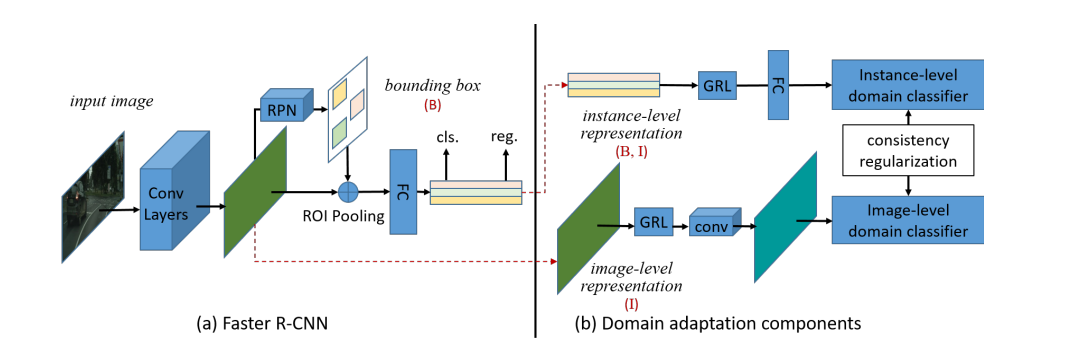
\includegraphics[width=16cm]{./faster_rcnn_DA.png}
	\end{center}
	\caption{Domain Adaptive Faster R-CNN for Object Detection in the Wild \cite{Chen2018}.}
	\begin{center}
		\label{Faster_rcnn_DA}
	\end{center}
\end{figure}
\FloatBarrier

Here, to maximize the domain classification losses $L_{inst}$ and $L_{img}$, they are calculated as shown in Equation \ref{faster_DA_losses}. 

\begin{equation}
\label{faster_DA_losses} 
\begin{gathered}
\mathcal{L}_{i m g}=-\sum_{i, u, v}\left[D_{i} \log p_{i}^{(u, v)}+\left(1-D_{i}\right) \log \left(1-p_{i}^{(u, v)}\right)\right] \\ 
\mathcal{L}_{i n s} = -\sum_{i, j}\left[D_{i} \log p_{i, j}+\left(1-D_{i}\right) \log \left(1-p_{i, j}\right)\right]
\end{gathered}
\cite{Chen2018}, 
\end{equation}
where $D_i=0$ is a ground-truth label of the sample image $i$ that originates from  the source domain and $D_i=1$ originates from the target domain; $p_{i,j}$ is a prediction output of the instance-level classifier for $j$-th proposed region of the sample image $i$; $p_{i}^{(u, v)}$ is a prediction output of the image-level domain classifier for the feature map region $(u,v)$ of a sample image $i$. 
Finally, two domain classifiers are regularized using consistency loss $\lambda \mathcal{L}_{\text {consistency }}$ as shown in Equation \ref{faster_DA_losses_consist}.  

\begin{equation}
\label{faster_DA_losses_consist} 
\mathcal{L}_{\text {consistency }}=\sum_{i, j}\left\|\frac{1}{|N|} \sum_{u, v} p_{i}^{(u, v)}-p_{i, j}\right\|_{2}
\cite{Chen2018}, 
\end{equation}
Due to the fact that the image-level domain classifier produces multiple $N$ predictions per image, first the average of them is calculated, and then the Euclidean (or L2 norm) distance is measured between the predictions of the image- and instance-level domain classifiers \cite{Chen2018}. 

The final objective of the network is then defined by minimizing the detection loss, while maximizing the image-level $\mathcal{L}_{img}$ and instance-level $\mathcal{L}_{inst}$ domain classification losses. The network additionally aims to minimize the consistency loss $\lambda \mathcal{L}_{\text {consistency }}$ between two classifiers \cite{Chen2018}.

Another most recent state-of-the-art study made by Rezaeianaran et al. \cite{Rezaeianaran2021} proposed different approach that compares the adversarial training to contrastive learning. Similarly to Chen et al. \cite{Chen2018}, the network leverages a Faster-RCNN detector with instance- and image-level alignments. Rezaeianaran et al. attempted a different approach by pushing the features closer if they represent the same class, and push them apart if otherwise. This is performed by utilizing a max-margin contrastive loss. The margin here denotes how far the features can be in order to be considered to represent the same class. A general constrastive loss term takes the form of Equation \ref{contrastiveL}:

\begin{equation}
\mathcal{L}_{C L}=\sum_{i}^{C}\left[\left\|F_{S}^{i}-F_{T}^{i}\right\|_{2}^{2}+\sum_{j, j \neq i}^{C} \max \left\{0, m-\left\|F_{S}^{i}-F_{T}^{j}\right\|_{2}^{2}\right\}\right]
\label{contrastiveL} 
\cite{Rezaeianaran2021} 
\end{equation}

Additionally, as the paper tried to solve UDA, no labels were available from the target domain and, therefore, pseudo-labeling was used to calculate the contrastive loss. \todo{This paper review should be rewritten} 


\begin{figure}[htb]
	\begin{center}
		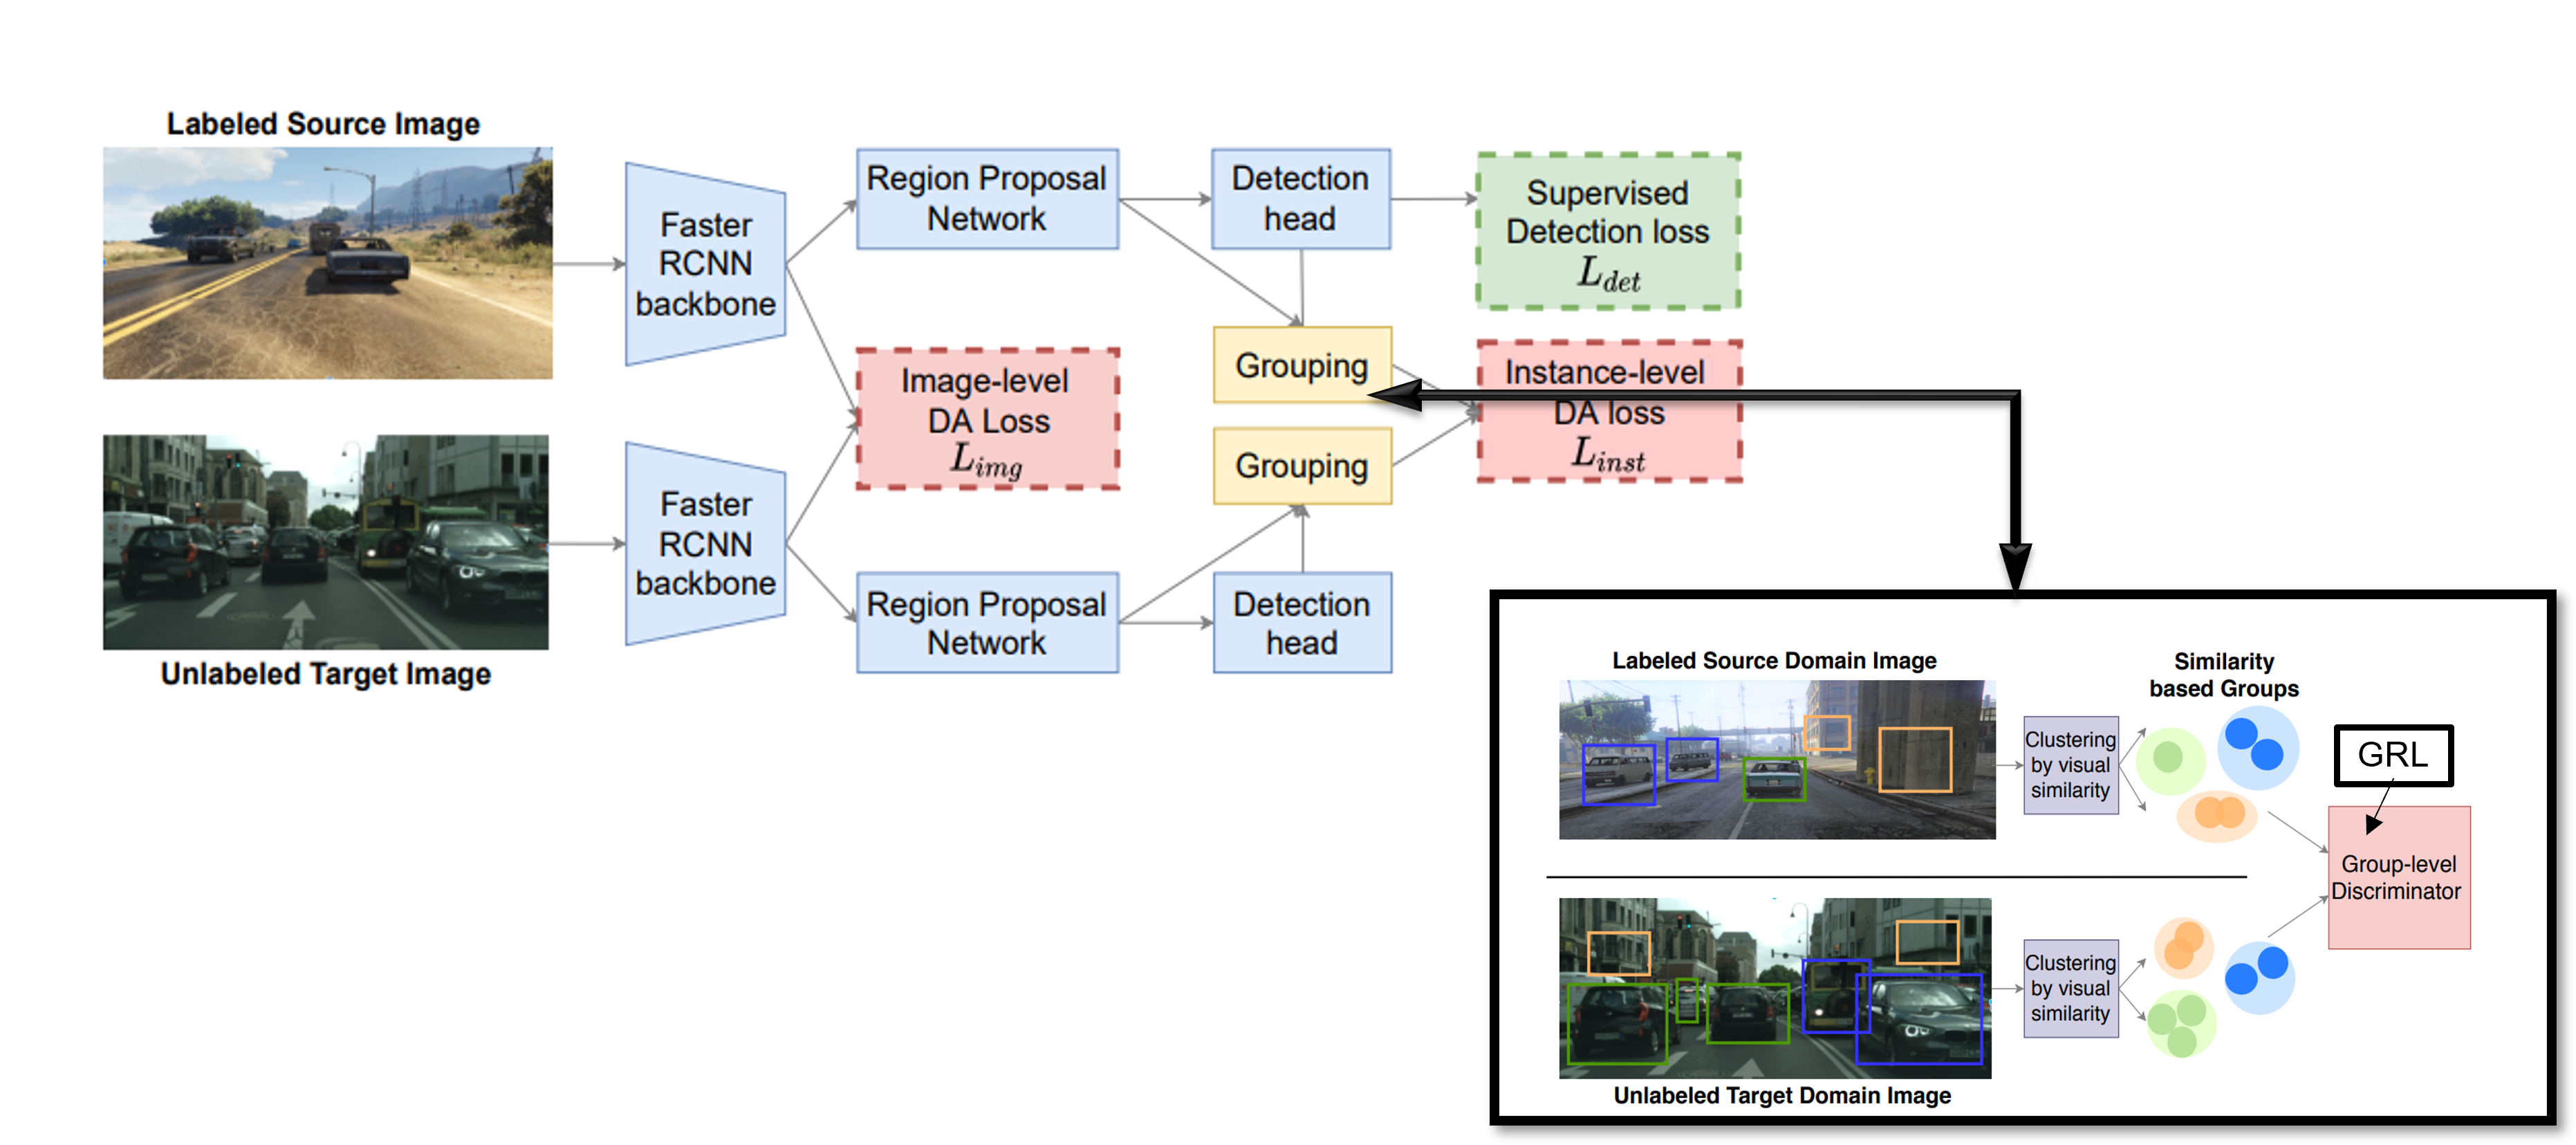
\includegraphics[width=16cm]{./VisGa.png}
	\end{center}
	\caption{Seeking Similarities over Differences: Similarity-based Domain Alignment for Adaptive Object Detection, adapted from \cite{Rezaeianaran2021}.}
	\begin{center}
		\label{visga}
	\end{center}
\end{figure}
\FloatBarrier


\subsubsection{Pseudo-labeling based methods}

Another relatively straightforward method to solve an object detection problem can be done by using pseudo-labels. A naive approach to pseudo-labeling is to first train the source dataset $\mathcal{D}_{\mathcal{S}}=\left\{\mathcal{X}_{\mathcal{S}}^{i}, \mathcal{Y}_{\mathcal{S}}^{i}\right\}_{i=1}^{\mathcal{N}_{\mathcal{S}}}$ and later run inference to obtain pseudo-labels on the target dataset $\mathcal{D}_{\mathcal{T}}=\left\{\mathcal{X}_{\mathcal{T}}^{j}\right\}_{j=1}^{\mathcal{N}_{\mathcal{T}}}$. The resulted labels will then form a new dataset $\dot{\mathcal{D}_{\mathcal{T}}}=\left\{\mathcal{X}_{\mathcal{T}}^{j}, \mathcal{Y}_{\mathcal{T}}^{j}\right\}_{j=1}^{\mathcal{N}_{\mathcal{T}}}$ \cite{Oza2021}. However, the results obtained will naturally be noisy and of poor quality. Khodabandeh et al. proposed a three-phase training process illustrated in Figure \ref{robust} below. 

\begin{figure}[htb]
	\begin{center}
		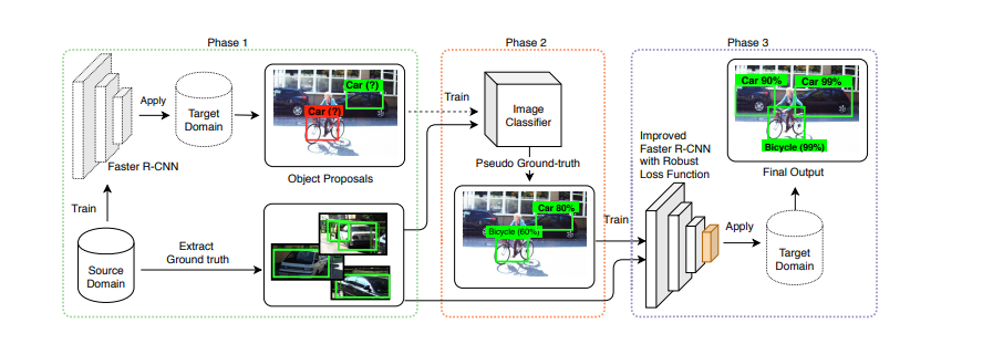
\includegraphics[width=16cm]{./robust.png}
	\end{center}
	\caption{A Robust Learning Approach to Domain Adaptive Object Detection \cite{Khodabandeh2019}.}
	\begin{center}
		\label{robust}
	\end{center}
\end{figure}
\FloatBarrier

In the first stage, the network is treated as a typical Faster-RCNN network that is trained on the source dataset $\mathcal{D_S}$. Next, the pseudo-labels are generated as explained earlier. In the following stage, the proposed regions are fed into a pre-trained image classifier, which allows to refine the model.

For the process of refinement, Khodabandeh et al. proposed to use the Kullback-Leibler divergence and defined the optimization objective for classification as follows: 

\begin{equation}
\min _{q} \operatorname{KL}\left(q\left(y_{c}\right) \| p_{c l s}\left(y_{c} \mid \boldsymbol{x}, \tilde{\boldsymbol{y}}_{l}\right)\right)+\alpha \operatorname{KL}\left(q\left(y_{c}\right)|| p_{i m g}\left(y_{c} \mid \boldsymbol{x}, \tilde{\boldsymbol{y}}_{l}\right)\right)
\label{KL_DV} 
\cite{Khodabandeh2019},
\end{equation}

where $y_c$ is the class label, $y_l$ is the bounding box location, $\alpha$ is a trade-off between two terms,  $p_{img}$ is the classification prediction of the image classification model and $p_{cls}$ is the classification prediction of the Faster-RCNN detector model. The goal of the refining process is to find a distribution $q(y_c)$ that is close to the models of $p_{cls}$ and $p_{img}$. The process is relatively similar for the bounding box refinement and the reader is advised to consult the original paper for more details \cite{Khodabandeh2019}.  

The third stage of the process finalizes the strategy by retraining the final network with the labeled ground truth data from $\mathcal{D_S}$ and the refined pseudo-labels from $\dot{\mathcal{D_T}}$. 


\subsubsection{Image-to-Image translation}
\label{imagetoimage} 
Another category that Oza et al. \cite{Oza2021} outlined is image-to-image translation for UDA. Instead of trying to align features, this group of methods essentially attempt to pull the domains together first. Hsu et al. \cite{Hsu2019} has suggested a Cycle-Generative Adversarial Network(GAN) \cite{Zhu2017} based approach to transform images from the target domain into the source domain alike images. Figure \ref{gan} represents the complete network proposed by Hsu et al. 

\begin{figure}[htb]
	\begin{center}
		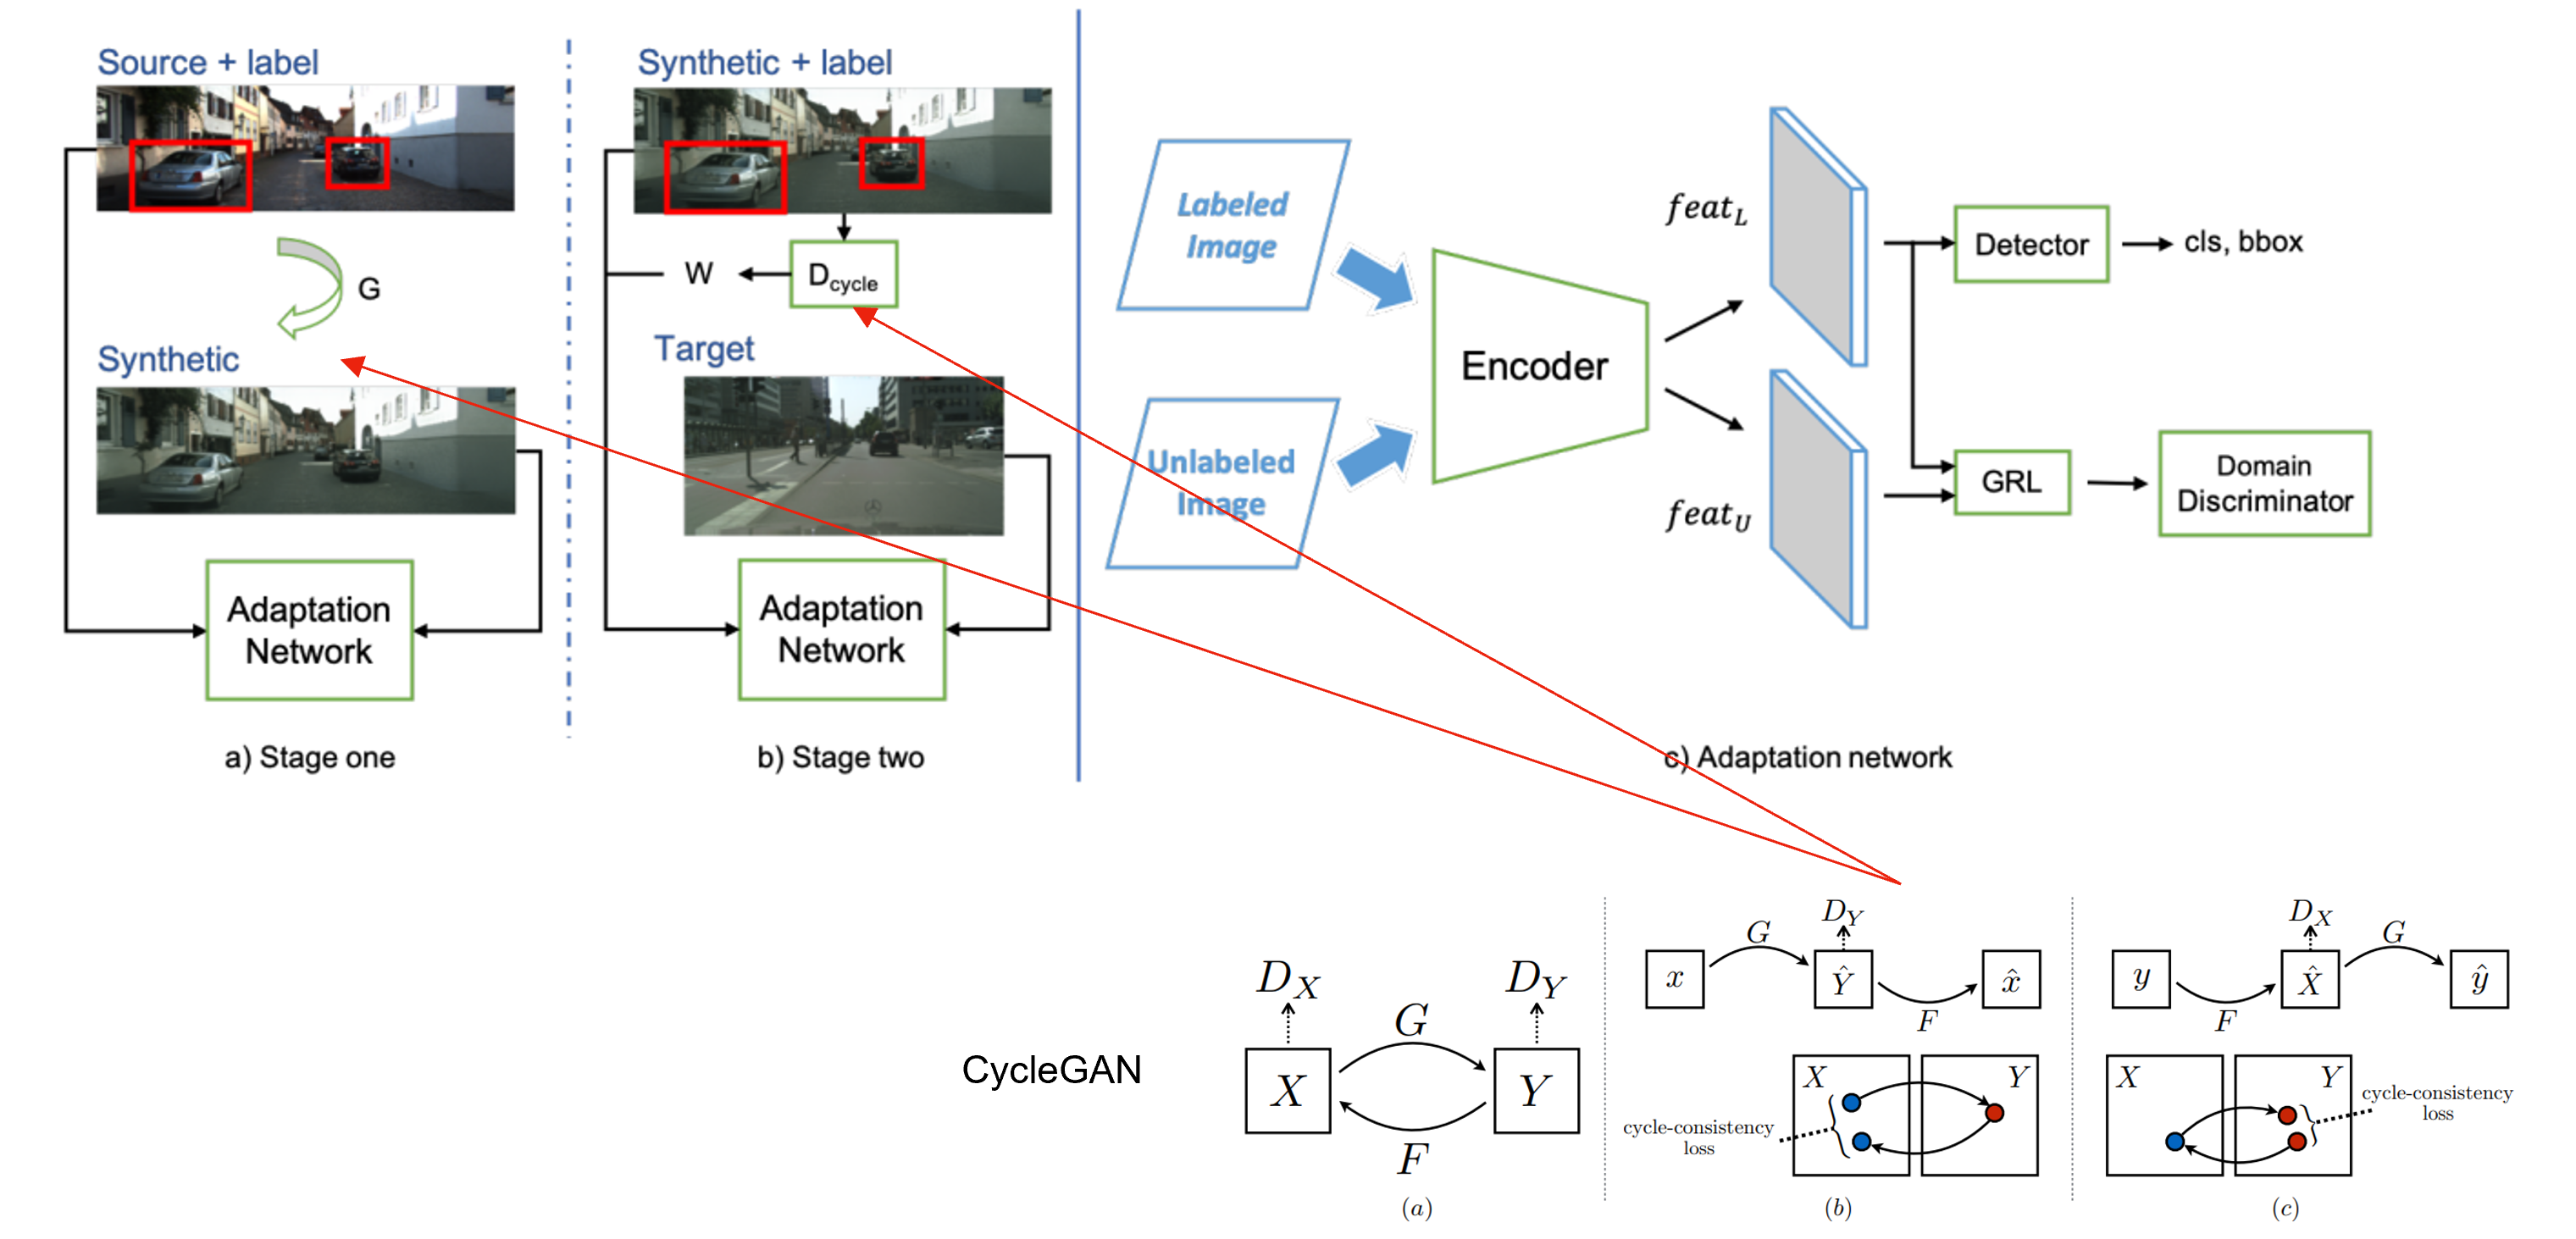
\includegraphics[width=16cm]{./GAN.png}
	\end{center}
	\caption{Progressive Domain Adaptation for Object Detection and CycleGAN, adapted from \cite{Hsu2019}.}
	\begin{center}
		\label{gan}
	\end{center}
\end{figure}
\FloatBarrier

The generator part of the Cycle-GAN in Figure \ref{gan} (a) creates intermediate domain from images in the source domain. The source images are then passed together with the labels to the Faster-RCNN network. The network is then tries to adapt the source domain to the synthetic domain. To further minimize the domain shift, adversarial learning techniques are used, such as a combination of a GRL and a domain classifier \cite{Hsu2019}.


In Figure \ref{gan} (b), the synthetic source-alike images are then passed together with the inherited source labels back to the adaptation network to align the features with the target domain. In the second stage of the training process, Hsu et al. proposed to utilize the weights $w$ from the discriminator of the Cycle-GAN, which is additionally trained to differentiate between source and target domains. Ultimately, such approach allowed to amplify the importance of the synthetic samples that are closer to the target domain. The weighted loss from the discriminator was then summed with the detection loss and the adversarial loss to finally adapt the synthetic domain to target \cite{Hsu2019}. 

\subsubsection{Domain randomization}

Oza et al. \cite{Oza2021} argues that often the accuracy of image-to-image translation methods is questionable as the domain shift between the synthetic and source domains still exists. Slightly different approach has been offered by Kim et al. \cite{Kim2019}. Instead of trying to pull two given domain distributions closer, they proposed a domain randomization technique, which generally attempts to generate a brand new domain that includes the same image in different style. This in practice allows the detector network to recognize features that are domain invariant and remove the domain bias. 

Kim et al. proposed a detector network that is based on Faster-RCNN with two additional components. The first component is a domain diversification module. Similarly to the method proposed by Hsu et al. \cite{Hsu2019}, the module leverages a Cycle-GAN \cite{Zhu2017}. However, the diversification module is used to generate images in a fixed set of new domains rather than to match the source dataset with target.  The second component is a multi-domain discriminator, which is essentially an adversarial feature learning approach, but instead of trying to confuse the detector in a binary set of domains, it tries to learn domain invariant features of multiple additional domains. The architecture of such domain randomization method is presented in Figure \ref{diversify}.

\begin{figure}[htb]
	\begin{center}
		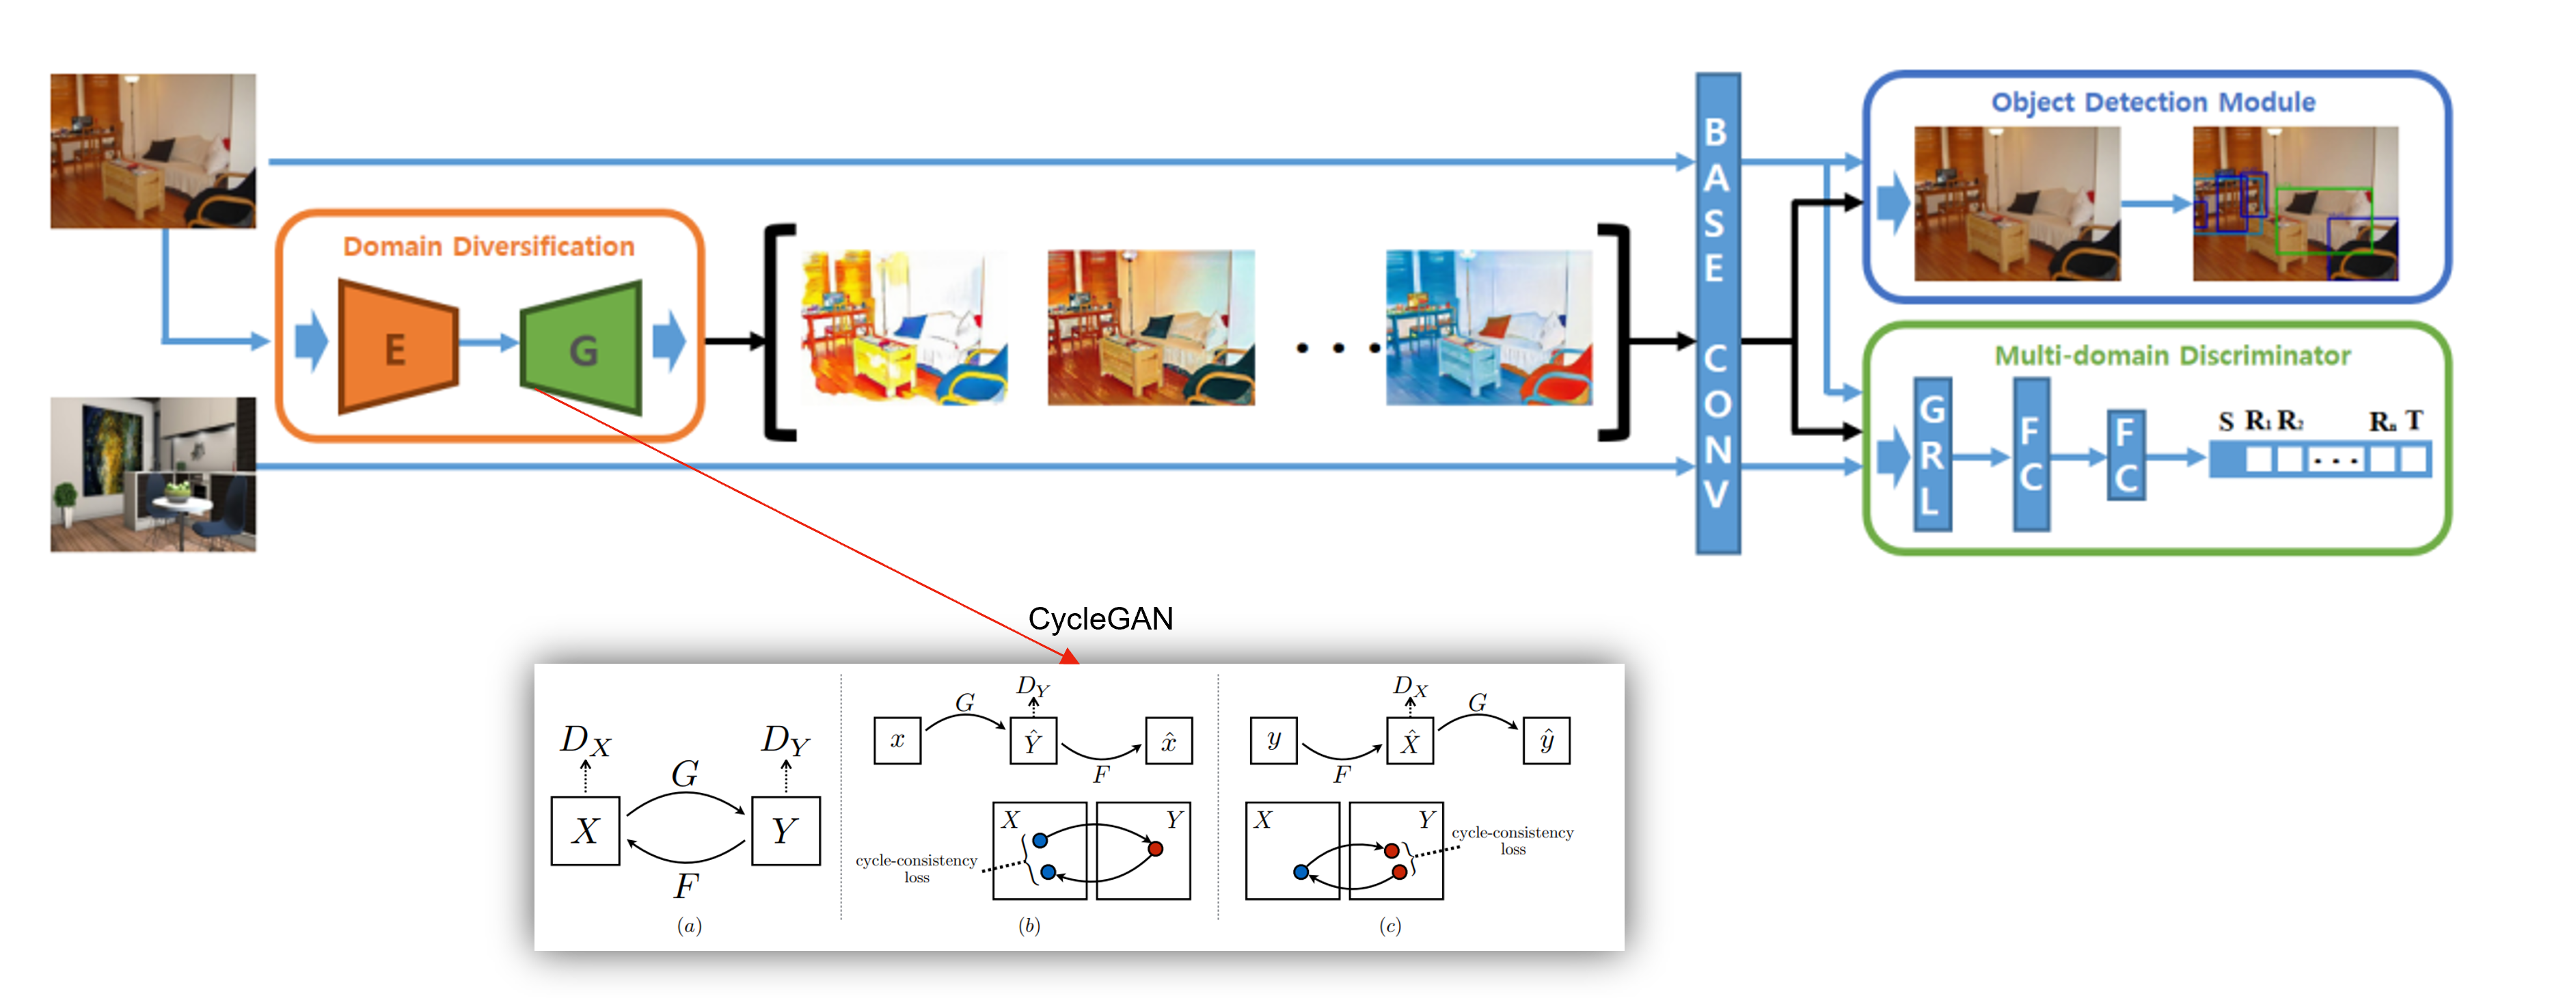
\includegraphics[width=16cm]{./diversify.png}
	\end{center}
	\caption{Diversify and Match: A Domain Adaptive Representation Learning Paradigm for Object Detection, adapted from \cite{Kim2019}.}
	\begin{center}
		\label{diversify}
	\end{center}
\end{figure}
\FloatBarrier

During Cycle-GAN image generation, two additional loss terms limited the  randomization of an image - color preservation and reconstruction constraints. This was done in order to preserve features of the original image as it would otherwise affect the model negatively \cite{Oza2021}. In the original experiments Kim et al. considered three additional domains: a color preserved domain, a reconstructed domain, and a domain that combines both. Images from all the domains are then fed into the detector along with the inherited source labels   to train a domain-invariant network with help of a multi-class domain classifier and the resulted model was used to verify performance on the target dataset. 

\subsubsection{Mean Teacher and Graph Reasoning}
\label{mean_teacher} 
Another common approach utilized in domain adaptation and transfer learning in general is mean teacher training. A typical mean teacher setup consists of two equivalent models. However, these models are trained using two separate strategies to adapt the detector network. On the other hand, graph reasoning based approaches of UDA have been gaining popularity not only in image classification problems, but also in object detectors. One potential reason for this is because graph models are easily applicable with other adaptation methodologies \cite{Oza2021}. Cai et al. \cite{Cai2019} proposed an architecture that combines both mean teacher and graph reasoning techniques in one solution and such architecture is presented in Figure \ref{graph_MT}. 
 
\begin{figure}[htb]
	\begin{center}
		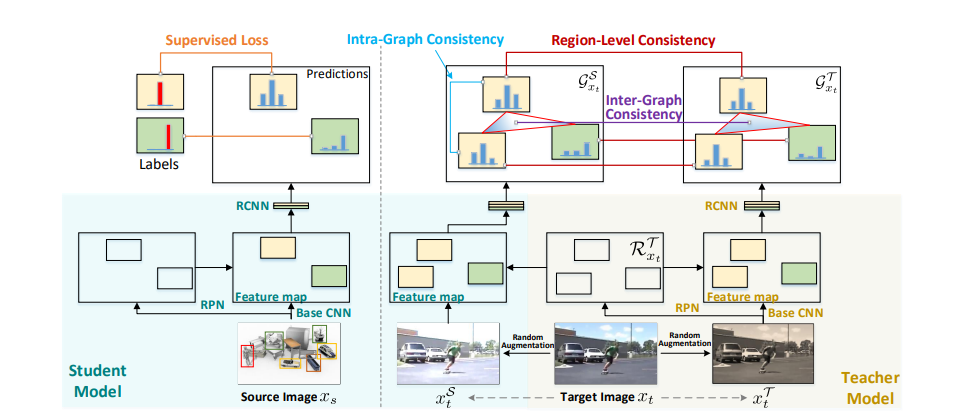
\includegraphics[width=16cm]{./graph_teacher.png}
	\end{center}
	\caption{Exploring Object Relation in Mean Teacher for Cross-Domain Detection \cite{Cai2019}.}
	\begin{center}
		\label{graph_MT}
	\end{center}
\end{figure}
\FloatBarrier

The term "graphs" represents a complex data structure that contains multiple nodes or vertices connected to each other via edges. In case of an image as a graph, each pixel can be considered a node, which is linked to all of its neighbors. 
The setup developed by Cai et al. \cite{Cai2019} introduces a student-teacher framework based on Faster-RCNN that verifies the consistency of the graphs at three different levels using regional-level consistency, intra-graph consistency and inter-graph consistency. 

The training pipeline is split into two parts. Images from the source domain are trained in a locked student environment in a supervised manner.  On the other hand, images from the target domain are augmented in two steps. First, the images are randomly cropped, padded or flipped. These images are passed through the pre-trained supervised student model that generates predictions. Meanwhile, the original target images are augmented with color jittering or corruption with noise. This set is send to the teacher model. The teacher model also produces predictions, which are then compared with the predictions from the first set of augmented images by utilizing region-level consistency. Essentially, the region-level consistency is calculated as MSE of the region-level prediction error in  both the student and the teacher. 

Inter-graph level consistency is used to verify the quality of the two graphs produced by the teacher and student models. It is calculated by means of cosine similarity between the graph representations of the proposed regions. 

Finally, intra-level consistency is then calculated to measure the quality of predictions within the same class of the student model. However, since target domain has no labels included in the UDA setup, the closest prediction $\operatorname{argmin} (labels)$ is used to produce pseudo-labels. The intra-level consistency loss is then calculated for any two instances of the same class in one graph. For more detailed calculation of the loss terms the readers are referred to the original paper by Cai et al. \cite{Cai2019}.

A purely mean-teacher-based semi-supervised approach has been proposed by Liu et al. \cite{Liu2021} As it can be seen from the overview illustrated in Figure \ref{unbiased}, it consists of two sequential stages. During the burn-in stage, Faster-RCNN detector is trained on the labeled data as normal. Next, the training pipeline is split into two equivalent Faster-RCNN-based detectors. The teacher model is supplied with weakly-augmented data. On the other hand, strongly-augmented images are fed into the student model. According to Liu et al., the main reason for that was because while strong augmentation is needed to improve performance of the model, the weaker augmentations were still needed in the teacher model to generate reliable pseudo-labels. These pseudo-labels are in turn used in the student model.   
\begin{figure}[htb]
	\begin{center}
		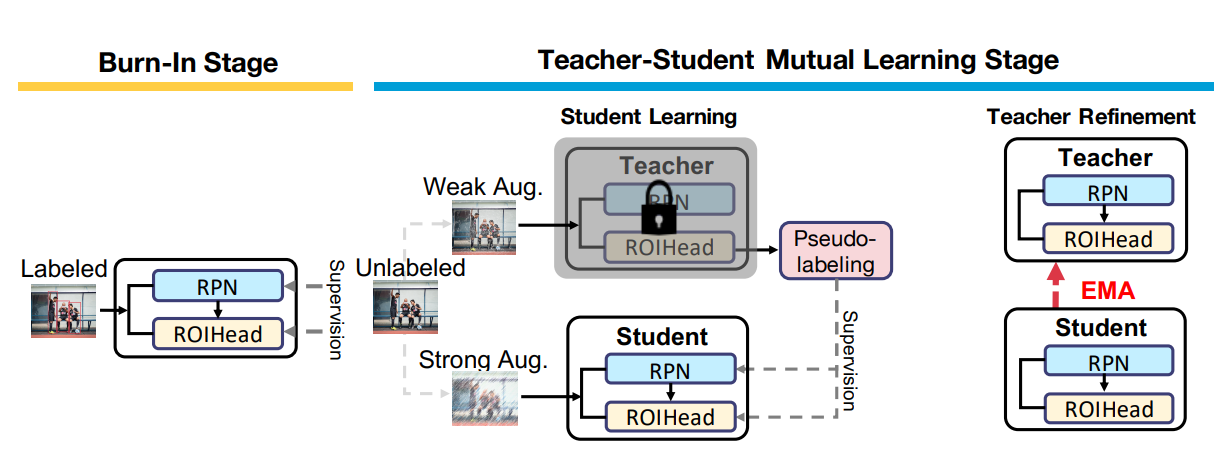
\includegraphics[width=14cm]{./unbiased.png}
	\end{center}
	\caption{Unbiased Teacher for Semi-Supervised Object Detection \cite{Liu2021}.}\label{unbiased}
	\begin{center}
	\end{center}
\end{figure}
\FloatBarrier

In order to achieve higher accuracy of pseudo-labels, the unbiased teacher model includes an Exponential Moving Average(EMA) module, along with a few other techniques \cite{Liu2021}. EMA attempts to emphasize the most recent data by granting it a higher weight. The EMA in Unbiased teacher is defined as follows: 
\begin{equation}
\theta_{t}^{i}=\hat{\theta}-\gamma \sum_{j=1}^{i-1}\left(1-\alpha^{-j+(i-1)}\right) \frac{\partial\left(\mathcal{L}_{\text {sup }}+\boldsymbol{\lambda}_{u} \mathcal{L}_{u n s u p}\right)}{\partial \theta_{s}^{j}}
\label{EMA}
\cite{Liu2021},
\end{equation}

where $\hat{\theta}$ is the initial (burn-in stage) model weight, $\theta_{t}^{i}$ is the weight of the teacher model, $\theta_{s}^{j}$ is the weight of the student model  at $i$-th and $j$-th iterations respectively. The weight of EMA in the training process is defined by $\alpha$ and $\gamma$ is the learning rate(LR) of the ensembled model \cite{Liu2021}.

Liu et al. also discusses the class imbalance problem that often causes the detector to learn underrepresented classes poorly \cite{Liu2021}. In order to solve this problem, Liu et al. propose to make use of the multi-focal loss \cite{Lin2017}, which attempts to put more weight on the samples with lower confidence, unlike a generic cross-entropy loss that treats all samples equally. 

However, this method only solves a semi-supervised object detection without addressing the domain shift issue. Expanding the unbiased teacher method, Li et al. \cite{Li2021} proposed to utilize mean teacher training in a domain adaptation setup. In addition to the original ensembled network proposed by Liu et al.  \cite{Liu2021}, adaptive teacher architecture employs adversarial feature learning techniques to adapt the target domain to the source. A typical domain adaptation network, which includes a GRL and a domain classifier, is appended to the backbone feature extractor of the student model. The complete architecture is displayed in Figure \ref{adapt_teacher}. 
 
\begin{figure}[htb]
	\begin{center}
		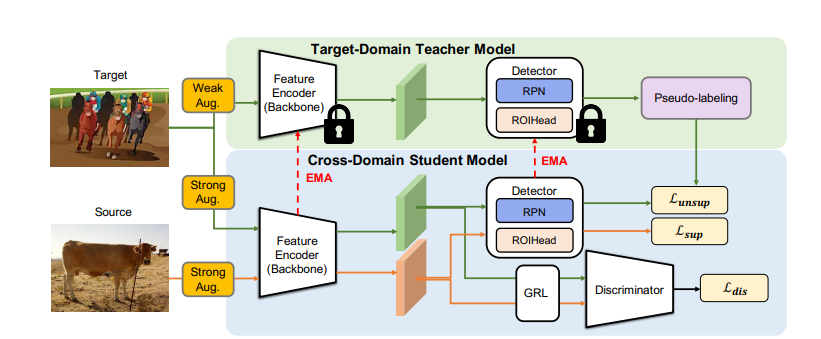
\includegraphics[width=16cm]{./adapt_teacher.png}
	\end{center}
	\caption{Cross-Domain Adaptive Teacher for Object Detection
\cite{Li2021}.}
	\begin{center}
		\label{adapt_teacher}
	\end{center}
\end{figure}
\FloatBarrier

Liu et al. \cite{Liu2021} specified that the teacher model is supplied with weakly-augmented target images, while the student model uses both strongly-augmented source and target images. Weak augmentations include cropping and flipping the image horizontally, and strong augmentations included grayscaling, color jittering, Gaussian blurring and cutting out patches. The same strategy was employed in this adaptive teacher method. The augmentations used in these works  \cite{Li2021, Liu2021} are presented in Figure \ref{augmentations}. 
\begin{figure}[htb]
	\begin{center}
		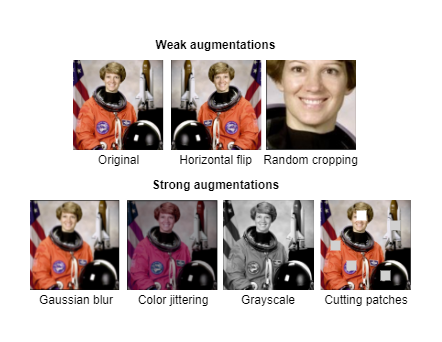
\includegraphics[width=10cm]{./augmentations.png}
	\end{center}
	\caption{Augmentations used in Unbiased teacher (adapted from the official Pytorch documentation \cite{pytorch}).}
	\begin{center}
		\label{augmentations}
	\end{center}
\end{figure}


Although all of the methods discussed in this chapter are based on the two-stage object detector Faster-RCNN, fewer papers also addressed a single-stage object detection in a domain adaptation setup, such as UDA for YOLO \cite{Hnewa2021}, \cite{Zhang2021a}, UDA for FCOS \cite{fcos1} and UDA for DETR \cite{Zhang2021b}, \cite{Vidit2021}. However, their review will be omitted with the grounds for it given in the \nameref{Methodology} section. 

\subsection{Continual learning}
\label{cont_learning} 
While transfer learning attempts to apply knowledge collected from one domain to another, lifelong learning offers adaptive algorithms, which  would accept a continuous stream of information that becomes available over time \cite{Parisi2018}. In case of the simple object detection problem, continual learning can be applied to a new task, such as to learn new classes of objects that are supplied progressively over time. This approach is potentially useful due to the scalability benefits it brings, since retraining the entire model every time a new object arrives to the database is computationally expensive. 

Similarly to the human brain, ANNs in object detectors tend to forget old knowledge learned as the memory gets overwritten with fresh data. This phenomenon in continual learning is commonly addressed as "catastrophic forgetting" \cite{Parisi2018}. Parisi et al. summarizes the up-to-date methods of continual learning that are effective against catastrophic forgetting into three categories: retraining with regularization, selective training with network expansion and retraining selective network with expansion. These methods are illustrated in Figure \ref{continual}. 

\begin{figure}[htb]
	\begin{center}
		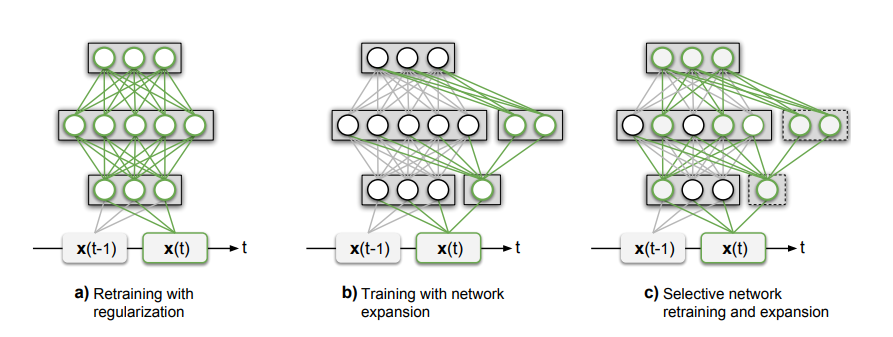
\includegraphics[width=16cm]{./continual.png}
	\end{center}
	\caption{Continual learning approaches
\cite{Parisi2018}.}
	\begin{center}
		\label{continual}
	\end{center}
\end{figure}
\FloatBarrier

The methods proposed in Figure \ref{continual} (a) attempt to solve catastrophic forgetting by means of regularization. In these group of methods, the algorithm seeks to penalize the modifications in the model of the originally trained task. A simplistic approach of such method was presented by Razavian et al.  \cite{Razavian2014}, where the gradients calculation for the parameters of the original is disabled completely. Slightly modified version of this method was also proposed by Donahue et al. \cite{Donahue2013}, where the LR was decreased to minimize the parameter update instead of blocking the update altogether. 


In simplistic terms, the method of training with expansion denotes retraning the original network with an additional number of layers appended. A typical example of such a method was proposed by Rusu et al. \cite{Rusu2016}, where the network was trained on the initial task. As $N$ new tasks were added, $N$ number of layers were appended to the network, as shown in Figure \ref{continual} (b). The parameters of the original network were left unchanged, and only the additional connections were trained. Although the disadvantage of this method was that the network complexity would grow linearly over time as new tasks are added, the experiments delivered sufficient performance. 

The method proposed by Yoon et al. \cite{Yoon2017} falls into the third category, which is illustrated in Figure \ref{continual} (c). The concept is fundamentally similar to the one suggested by Rusu et al. \cite{Rusu2016}, with the exception that their model selectively retrains the network from the original task. Connecting the neurons sparsely reduced the computational overhead, as well as allowed the network to retain the previously learned tasks. Parisi et al. \cite{Parisi2018} have collected many other promising continual learning methods and the reader is advised to refer to the original survey for more details.   

In the context of the notation defined earlier in the \nameref{transferLearning} subsection, continual learning can be expressed as training on the task $\mathcal{T}_n$ given the task $\mathcal{T}_{n-1}$ within the same domain or a set of domains $\mathcal{D}_{n} = \mathcal{D}_{n-1}$.   

\todo{perhaps add the final CL graph from Parisi2018} 


\clearpage 